\chapter{Resultados}
\label{c.resultados}
Ao executar o script, a simulação foi salva em dois arquivos de texto. O primeiro, representado no quadro \ref{q.res1}, demonstra a probabilidade de chuva para todos os 365 dias do ano de 2021. O segundo arquivo, representado no quadro \ref{q.res2}, e também foco principal do trabalho, mostra se os dias vão ser chuvosos ou não. Para isso, utiliza o numero 1 e 0 se forem chuvosos ou secos, respectivamente. As colunas representam os meses, de janeiro a dezembro, com um total de 12 colunas. De forma similar, as linhas representam os dias, de 1 a 31, com um total de 31 linhas.

\begin{table}[H]
\caption{Resultado da simulação com as probabilidades condicionais geradas pelo script.}
\label{q.res1}
\centering
\begin{tabular}{|c|c|c|c|c|c|c|c|c|c|c|c|}
\hline
0.5  & 0.07 & 0.08 & 0    & 0    & 0.08 & 0.13 & 0.06 & 0.42 & 0.5  & 0.2  & 0.64 \\ \hline
0.67 & 0.15 & 0.23 & 0.19 & 0.13 & 0.25 & 0.13 & 0.06 & 0    & 0.5  & 0.23 & 0.08 \\ \hline
0.9  & 0.56 & 0.17 & 0.75 & 0.5  & 0.71 & 0.06 & 0.13 & 0.06 & 0.6  & 0.08 & 0.33 \\ \hline
0.64 & 0.1  & 0.18 & 0.6  & 0.19 & 0.25 & 0.13 & 0.06 & 0.13 & 0.5  & 0.36 & 0.25 \\ \hline
0.7  & 0.08 & 0.08 & 0.5  & 0.23 & 0.4  & 0    & 0.06 & 0.06 & 1    & 0.08 & 0.36 \\ \hline
0.25 & 0.33 & 0.27 & 0.57 & 0    & 0.75 & 0.06 & 0.06 & 0.06 & 0.25 & 0.25 & 0.36 \\ \hline
1    & 0.56 & 0.17 & 0.23 & 0    & 0.6  & 0.06 & 0.12 & 0.13 & 0.2  & 0.5  & 0.6  \\ \hline
1    & 0.75 & 0.25 & 0.07 & 0.29 & 0.07 & 0.13 & 0.06 & 0.06 & 0.17 & 0.5  & 0.8  \\ \hline
0.5  & 0.75 & 0.14 & 0.14 & 0.25 & 0    & 0.06 & 0    & 0.06 & 0.5  & 0.4  & 0.33 \\ \hline
0.11 & 0.56 & 0.21 & 0.2  & 0.06 & 0.38 & 0.33 & 0    & 1    & 0.08 & 0.36 & 0.63 \\ \hline
0.44 & 0.22 & 0.45 & 0.67 & 0.06 & 0.13 & 0.36 & 0    & 0.33 & 0.06 & 0    & 0.3  \\ \hline
1    & 0.11 & 0.17 & 0.06 & 0.13 & 0.06 & 0.13 & 0    & 0    & 0.21 & 0.13 & 0.63 \\ \hline
0.75 & 0.5  & 0    & 0.36 & 0    & 0.13 & 0.12 & 0    & 0    & 0.6  & 0.36 & 0.18 \\ \hline
0.89 & 0.8  & 0.45 & 0.23 & 0.2  & 0.13 & 0.06 & 0.12 & 0.06 & 0.17 & 0.78 & 0.27 \\ \hline
0.55 & 0.7  & 0.6  & 0.14 & 0.15 & 0.06 & 0    & 0    & 0    & 0.18 & 0.8  & 0.89 \\ \hline
0.67 & 0.73 & 0.17 & 0.21 & 0.25 & 0.31 & 0.12 & 0.12 & 0.19 & 0.15 & 0.5  & 0.71 \\ \hline
0.77 & 0.9  & 0.07 & 0.06 & 0.07 & 0    & 0.06 & 0.06 & 0.06 & 0.14 & 0    & 0.63 \\ \hline
0.9  & 0.38 & 0.23 & 0    & 0.2  & 0    & 0.2  & 0.06 & 0.06 & 0.29 & 0.31 & 0.07 \\ \hline
0.78 & 0.5  & 0.2  & 0.06 & 0.38 & 0.12 & 0.07 & 0.06 & 0.19 & 0.31 & 0.25 & 0.5  \\ \hline
0.75 & 1    & 0.42 & 0.13 & 1    & 0.13 & 0.06 & 0.13 & 0.36 & 0.4  & 0.15 & 0.44 \\ \hline
0.8  & 0.55 & 0.5  & 0.31 & 0.75 & 0    & 0.06 & 0.07 & 0.08 & 0.27 & 0.13 & 0.67 \\ \hline
0.56 & 0.8  & 0.44 & 0.23 & 0.23 & 0.14 & 0.2  & 0    & 0.2  & 0.38 & 0.42 & 0.45 \\ \hline
0.75 & 0.75 & 0.17 & 0.67 & 0.33 & 0    & 0.06 & 0.06 & 0.06 & 0.17 & 1    & 0.88 \\ \hline
0.3  & 0.36 & 0.15 & 0.2  & 0.17 & 0.06 & 0    & 0    & 0.19 & 0.14 & 0.2  & 0.58 \\ \hline
0.4  & 0.83 & 0.5  & 0.5  & 0.25 & 0.13 & 0.2  & 0.27 & 0.27 & 0.13 & 0.23 & 0.2  \\ \hline
0.57 & 0.86 & 0.33 & 0.13 & 0.75 & 0.4  & 0    & 0    & 0.25 & 0.45 & 0.36 & 0.44 \\ \hline
0.67 & 0.6  & 0.14 & 0.13 & 0.33 & 0    & 0    & 0.36 & 0    & 0.17 & 0.25 & 0.09 \\ \hline
0.85 & 0.67 & 0.13 & 0.13 & 0.4  & 0    & 0    & 0    & 0.07 & 0.56 & 0.14 & 0.25 \\ \hline
0.92 & -    & 0.06 & 0.12 & 0.43 & 0.06 & 0.06 & 0    & 0.06 & 0.06 & 0.33 & 0.29 \\ \hline
1    & -    & 0.29 & 0.29 & 0    & 0.06 & 0    & 0.06 & 0.2  & 0.64 & 0.06 & 0.18 \\ \hline
0.56 & -    & 0    & -    & 0.33 & -    & 0.06 & 0.12 & -    & 0.83 & -    & 0.8  \\ \hline
\end{tabular}
\vspace*{15px}
\legend{\small Fonte: Elaborado pelo autor.}
\end{table}


\begin{table}[H]
\caption{Resultado principal da simulação com os dados binários gerados pelo script.}
\label{q.res2}
\centering
\begin{tabular}{|c|c|c|c|c|c|c|c|c|c|c|c|}
\hline
1 & 0 & 0 & 0 & 0 & 0 & 0 & 0 & 0 & 1 & 0 & 0 \\ \hline
1 & 1 & 0 & 1 & 1 & 1 & 0 & 0 & 0 & 1 & 0 & 0 \\ \hline
1 & 0 & 0 & 1 & 0 & 0 & 0 & 0 & 0 & 1 & 0 & 0 \\ \hline
1 & 0 & 0 & 1 & 0 & 0 & 0 & 0 & 0 & 1 & 0 & 0 \\ \hline
0 & 0 & 0 & 1 & 0 & 1 & 0 & 0 & 0 & 1 & 0 & 0 \\ \hline
0 & 1 & 0 & 0 & 0 & 1 & 0 & 0 & 0 & 0 & 1 & 1 \\ \hline
1 & 1 & 0 & 0 & 0 & 0 & 0 & 0 & 0 & 1 & 1 & 1 \\ \hline
1 & 1 & 0 & 0 & 1 & 0 & 0 & 0 & 0 & 1 & 1 & 0 \\ \hline
0 & 1 & 0 & 0 & 0 & 0 & 1 & 0 & 1 & 0 & 0 & 1 \\ \hline
0 & 0 & 0 & 1 & 0 & 0 & 0 & 0 & 1 & 0 & 0 & 0 \\ \hline
0 & 0 & 0 & 0 & 0 & 0 & 0 & 0 & 0 & 0 & 0 & 1 \\ \hline
1 & 1 & 0 & 0 & 0 & 0 & 0 & 0 & 0 & 0 & 0 & 0 \\ \hline
1 & 1 & 0 & 0 & 0 & 0 & 0 & 0 & 0 & 0 & 1 & 0 \\ \hline
1 & 1 & 1 & 0 & 0 & 0 & 0 & 0 & 0 & 0 & 1 & 1 \\ \hline
0 & 1 & 0 & 0 & 1 & 0 & 0 & 0 & 0 & 0 & 1 & 1 \\ \hline
1 & 1 & 0 & 0 & 0 & 0 & 0 & 0 & 0 & 0 & 1 & 1 \\ \hline
1 & 0 & 0 & 0 & 0 & 0 & 0 & 0 & 0 & 0 & 0 & 0 \\ \hline
1 & 0 & 0 & 0 & 1 & 0 & 0 & 0 & 0 & 0 & 0 & 0 \\ \hline
1 & 1 & 0 & 0 & 1 & 0 & 0 & 0 & 0 & 1 & 0 & 1 \\ \hline
1 & 1 & 1 & 0 & 1 & 0 & 0 & 0 & 0 & 0 & 0 & 1 \\ \hline
1 & 1 & 0 & 0 & 0 & 0 & 0 & 0 & 0 & 1 & 0 & 1 \\ \hline
1 & 1 & 0 & 1 & 0 & 0 & 0 & 0 & 0 & 0 & 1 & 1 \\ \hline
0 & 0 & 0 & 0 & 0 & 0 & 0 & 0 & 0 & 0 & 1 & 1 \\ \hline
0 & 0 & 1 & 1 & 0 & 0 & 0 & 0 & 0 & 0 & 0 & 0 \\ \hline
0 & 1 & 1 & 0 & 1 & 1 & 0 & 0 & 0 & 0 & 0 & 0 \\ \hline
1 & 1 & 0 & 0 & 1 & 0 & 0 & 0 & 0 & 0 & 0 & 0 \\ \hline
1 & 1 & 0 & 0 & 1 & 0 & 0 & 0 & 0 & 0 & 0 & 0 \\ \hline
1 & 0 & 0 & 0 & 1 & 0 & 0 & 0 & 0 & 0 & 0 & 1 \\ \hline
1 & - & 0 & 0 & 0 & 0 & 0 & 0 & 0 & 0 & 0 & 0 \\ \hline
1 & - & 0 & 0 & 0 & 0 & 0 & 0 & 1 & 1 & 0 & 1 \\ \hline
0 & - & 0 & - & 0 & - & 0 & 0 & - & 0 & - & 1 \\ \hline
\end{tabular}
\vspace*{15px}
\legend{\small Fonte: Elaborado pelo autor.}
\end{table}

\section{Análise mês a mês}

\subsection{Janeiro}
\begin{figure}[H]
	\caption{\small Chuva x Dia - Janeiro/2021}
	\centering
	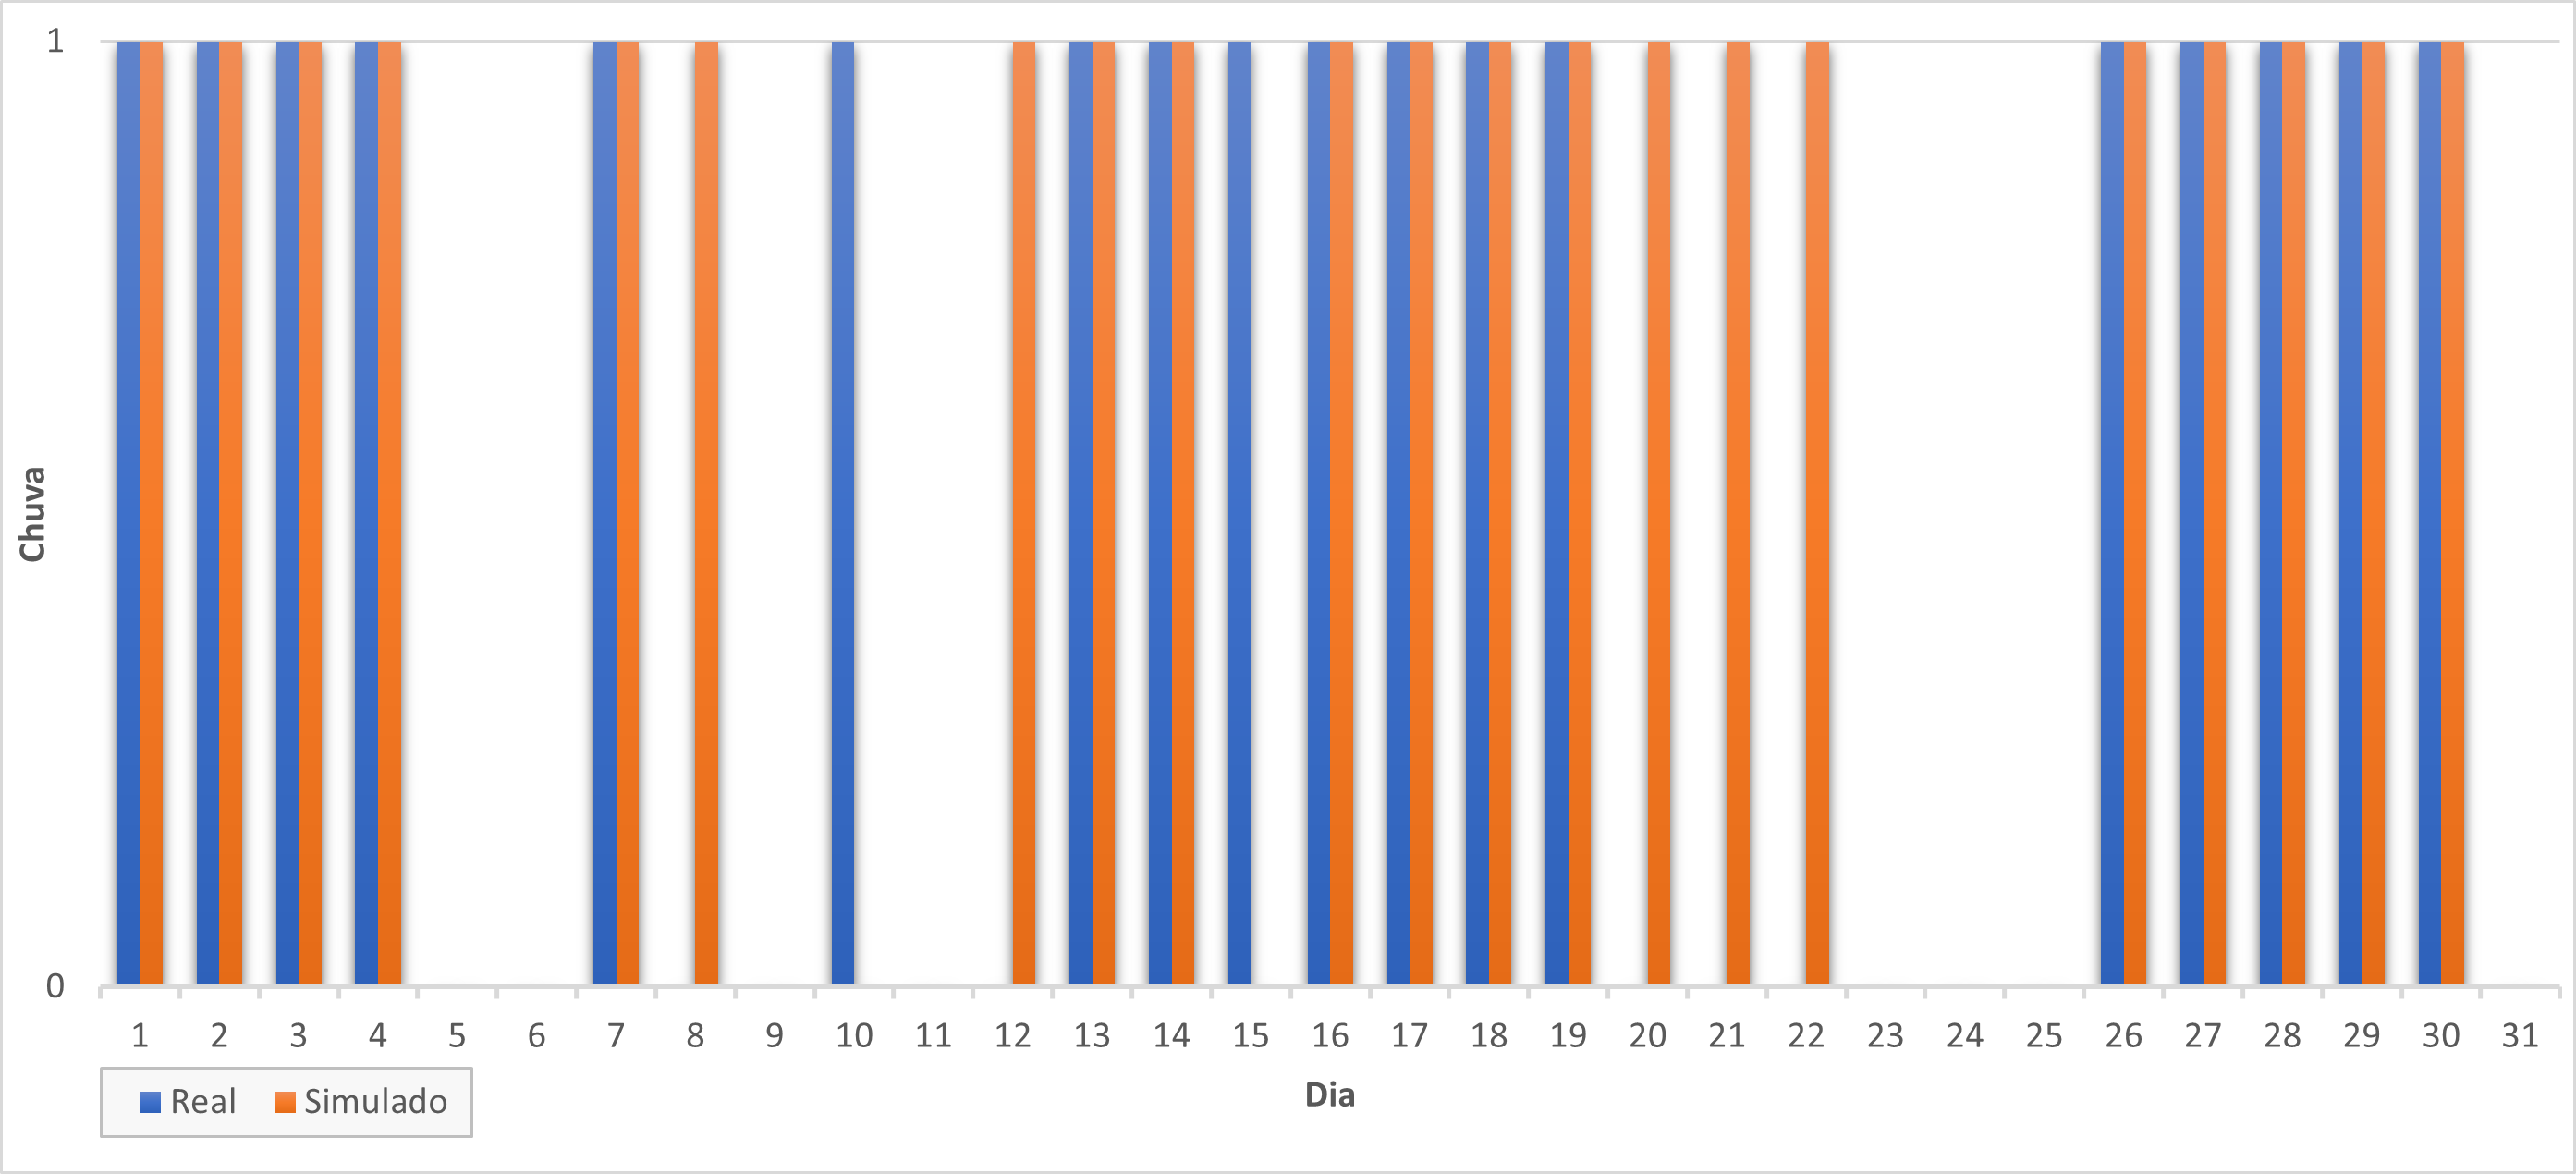
\includegraphics[width=\textwidth]{figs/jan.png}
	\label{f.rjan}
	\legend{\small Fonte: Elaborado pelo autor.}
\end{figure}

\subsection{Fevereiro}
\begin{figure}[H]
	\caption{\small Chuva x Dia - Fevereiro/2021}
	\centering
	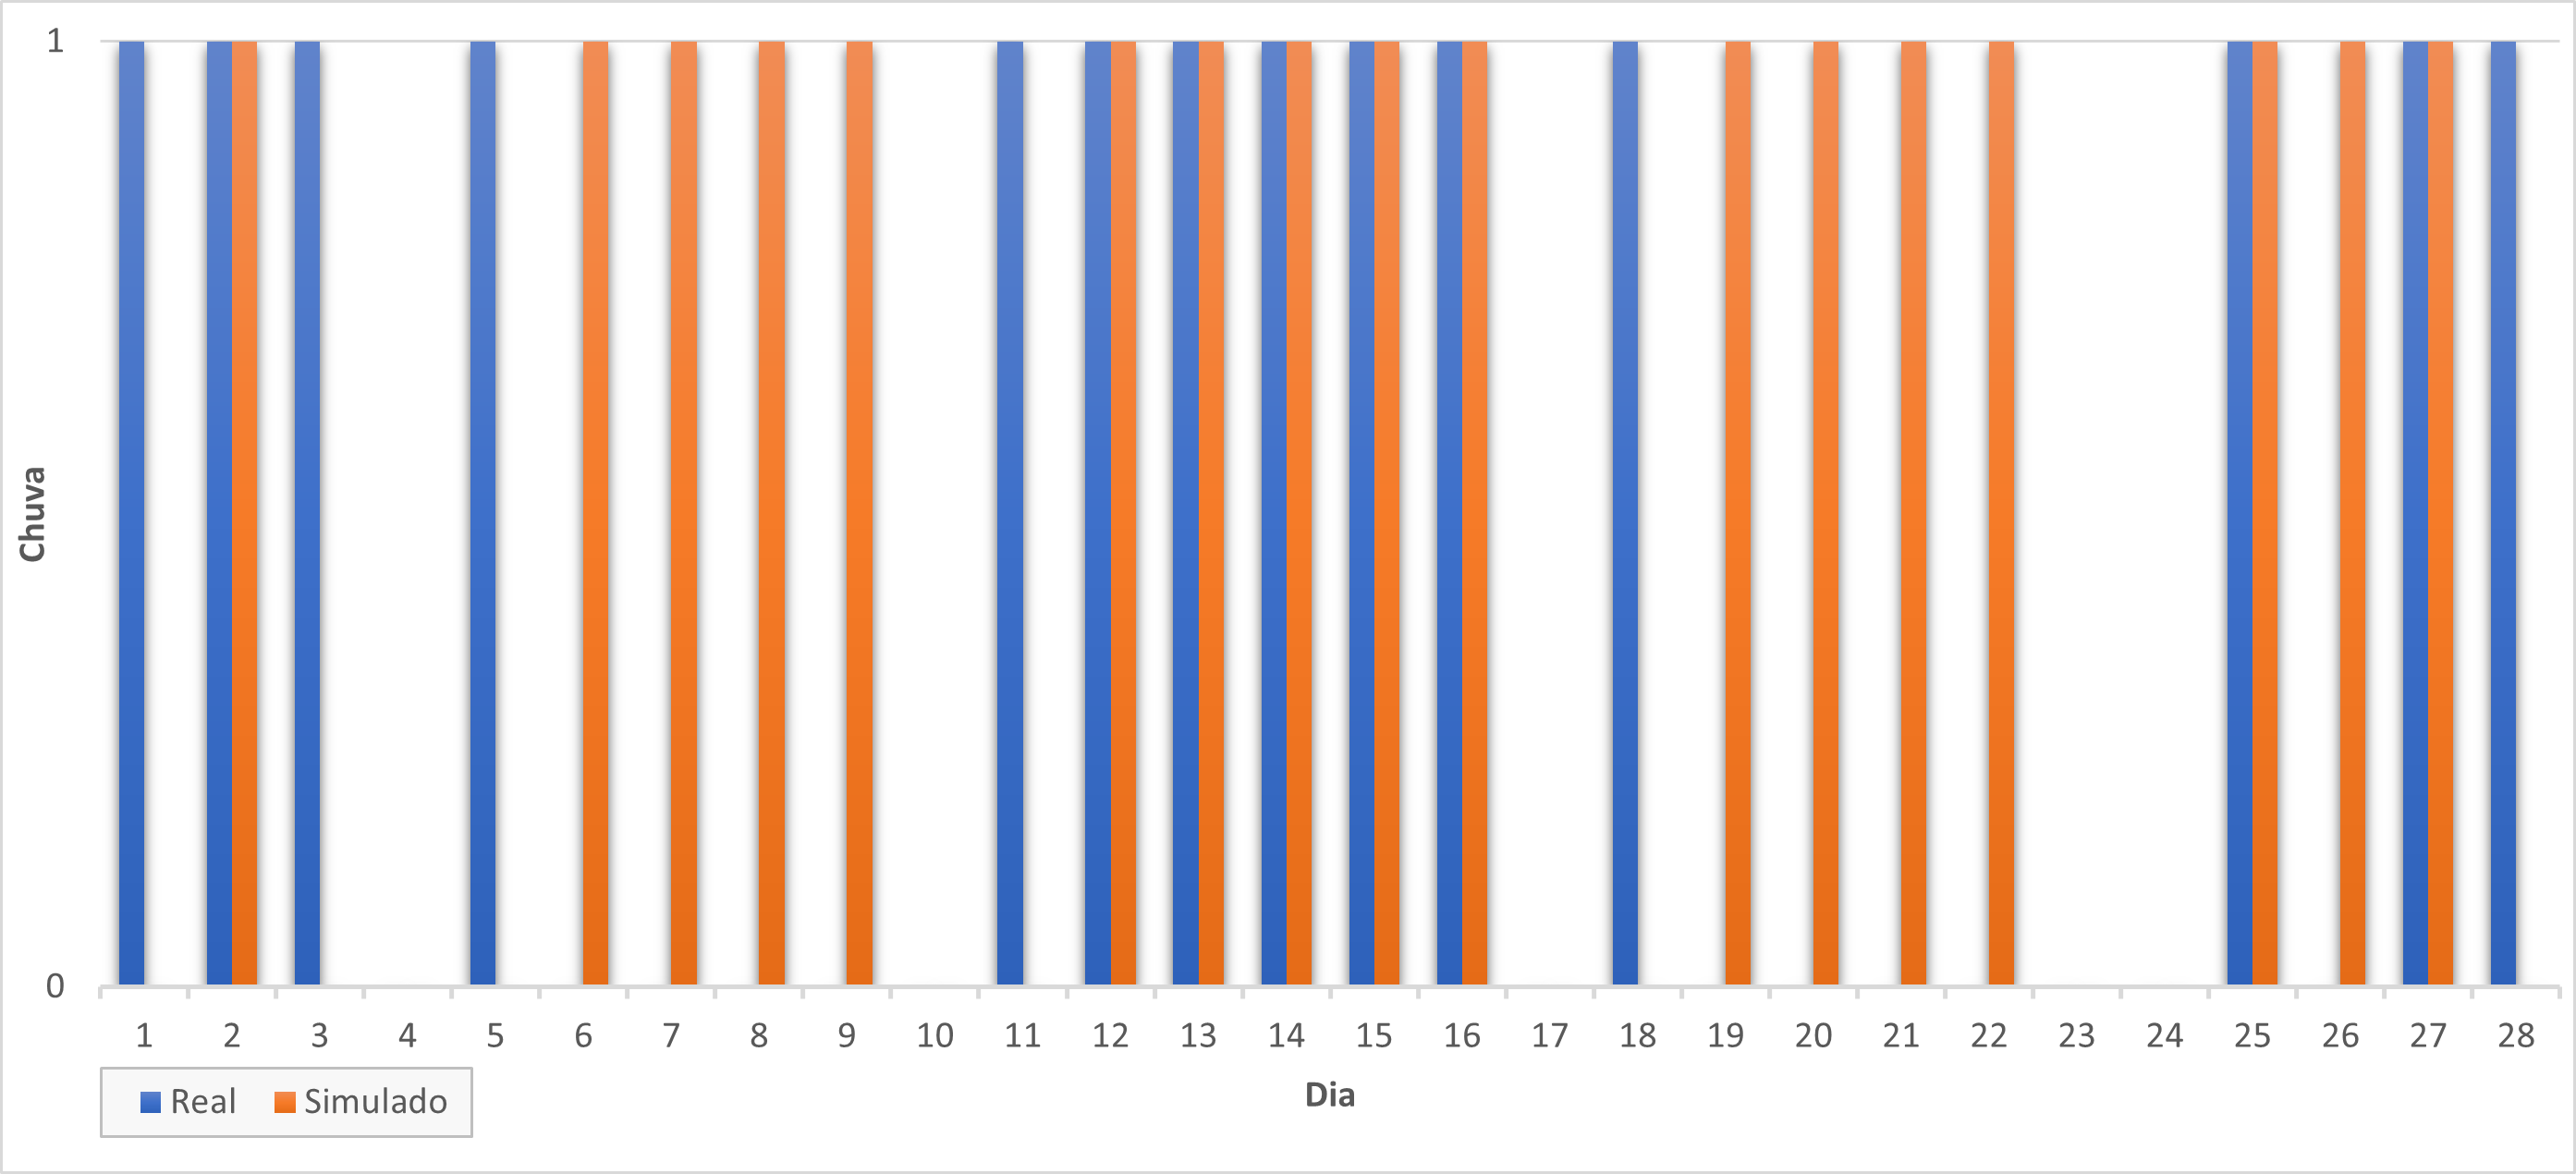
\includegraphics[width=\textwidth]{figs/fev.png}
	\label{f.rfev}
	\legend{\small Fonte: Elaborado pelo autor.}
\end{figure}

\subsection{Marco}
\begin{figure}[H]
	\caption{\small Chuva x Dia - Março/2021}
	\centering
	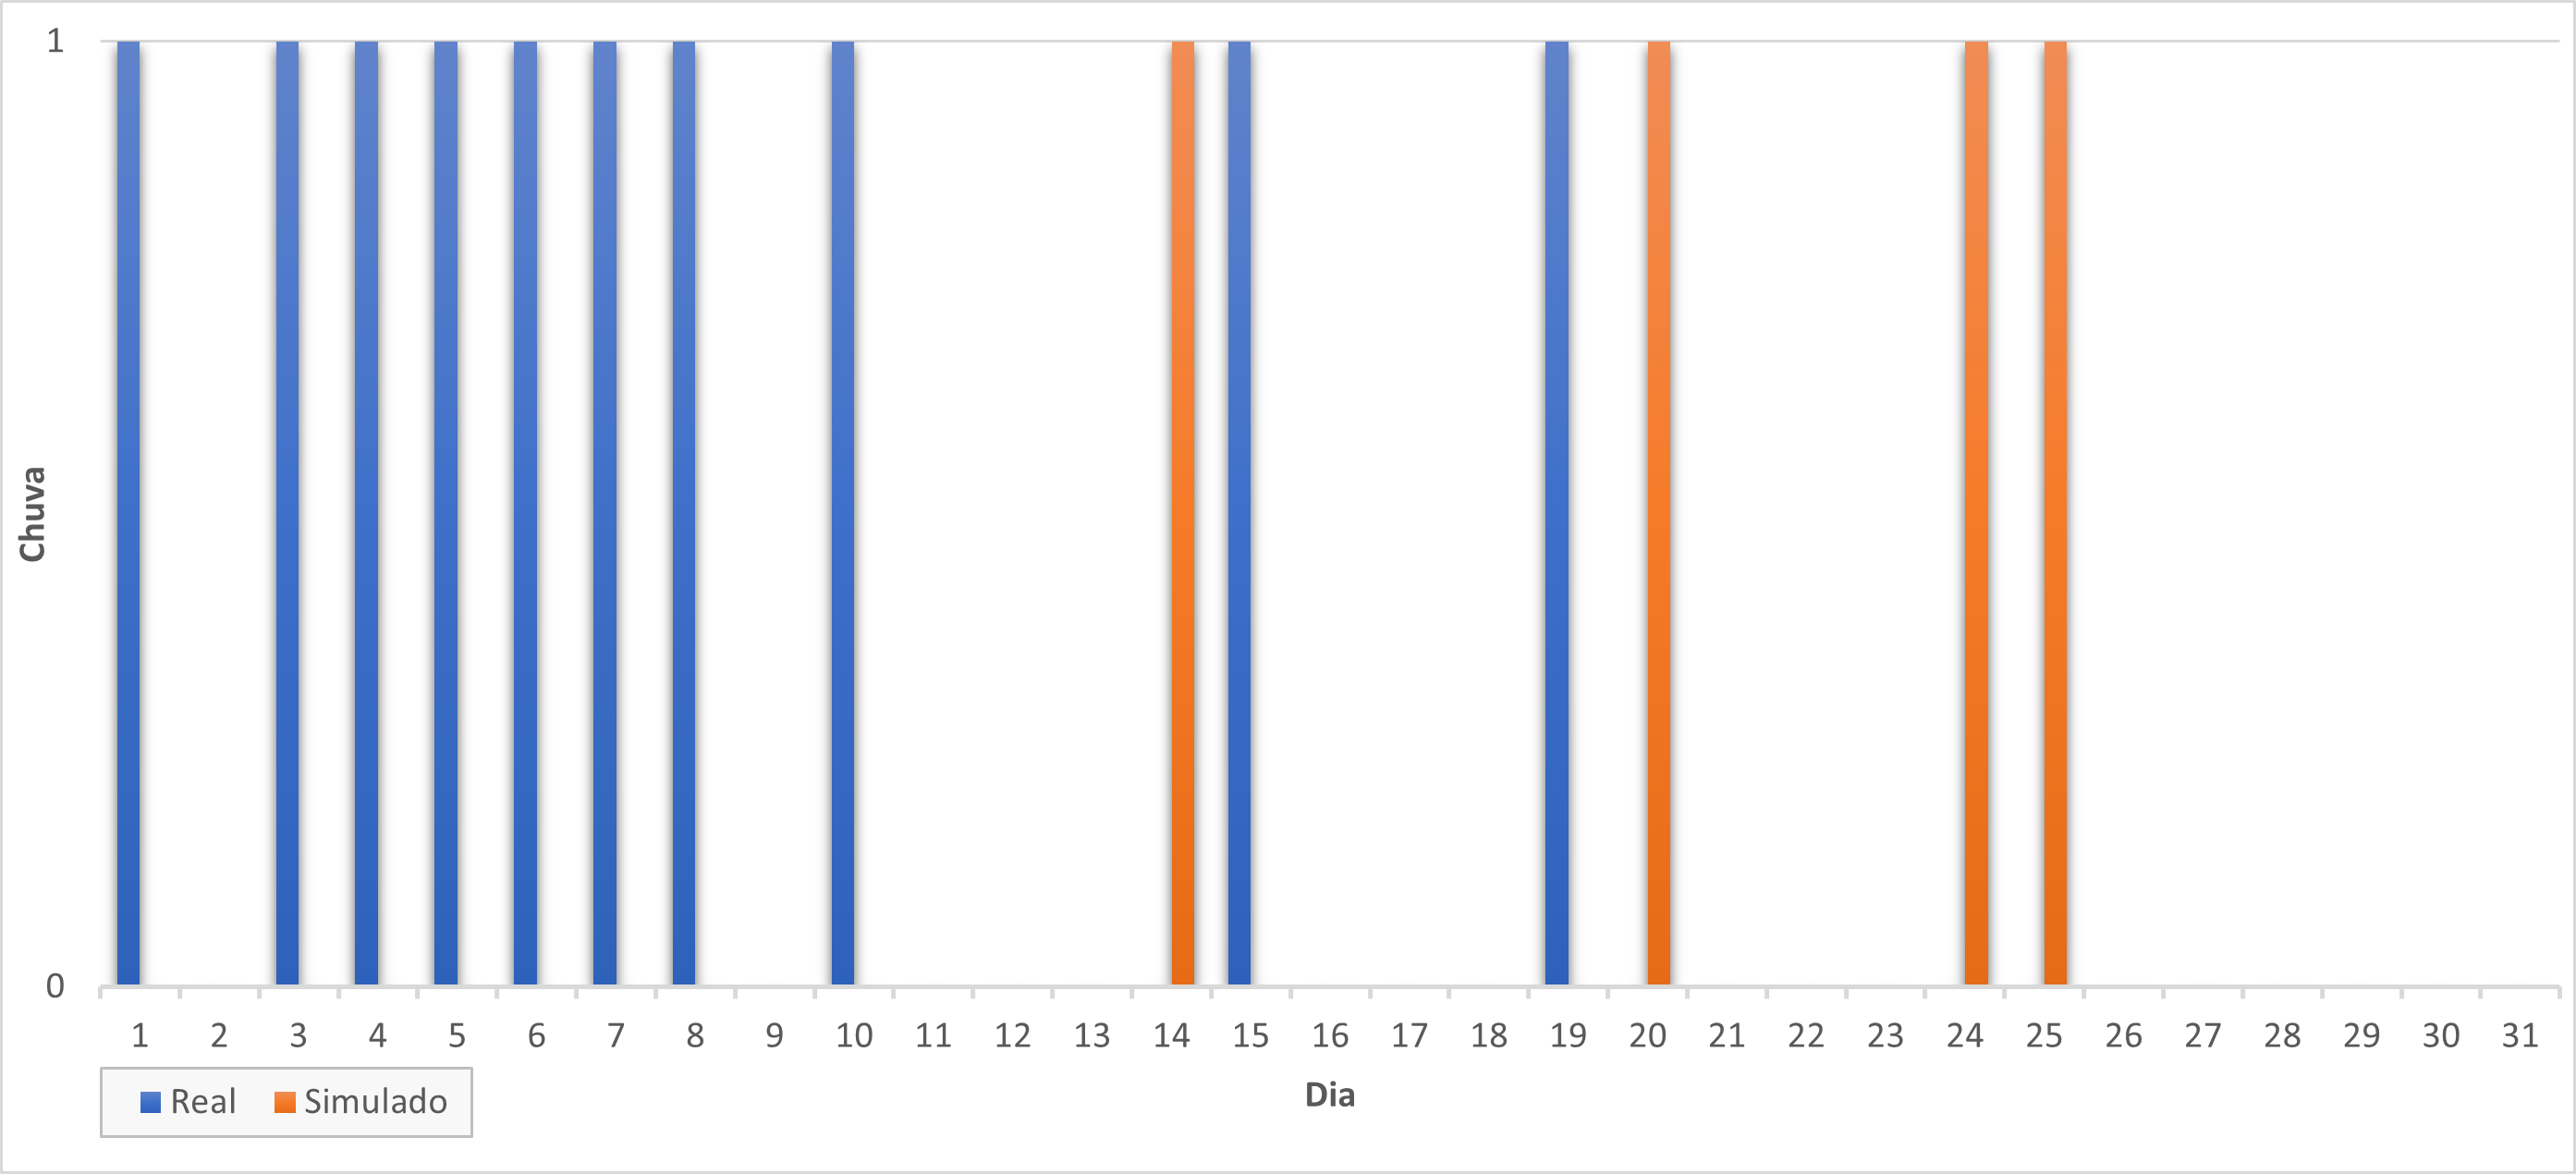
\includegraphics[width=\textwidth]{figs/mar.png}
	\label{f.rmar}
	\legend{\small Fonte: Elaborado pelo autor.}
\end{figure}

\subsection{Abril}
\begin{figure}[H]
	\caption{\small Chuva x Dia - Abril/2021}
	\centering
	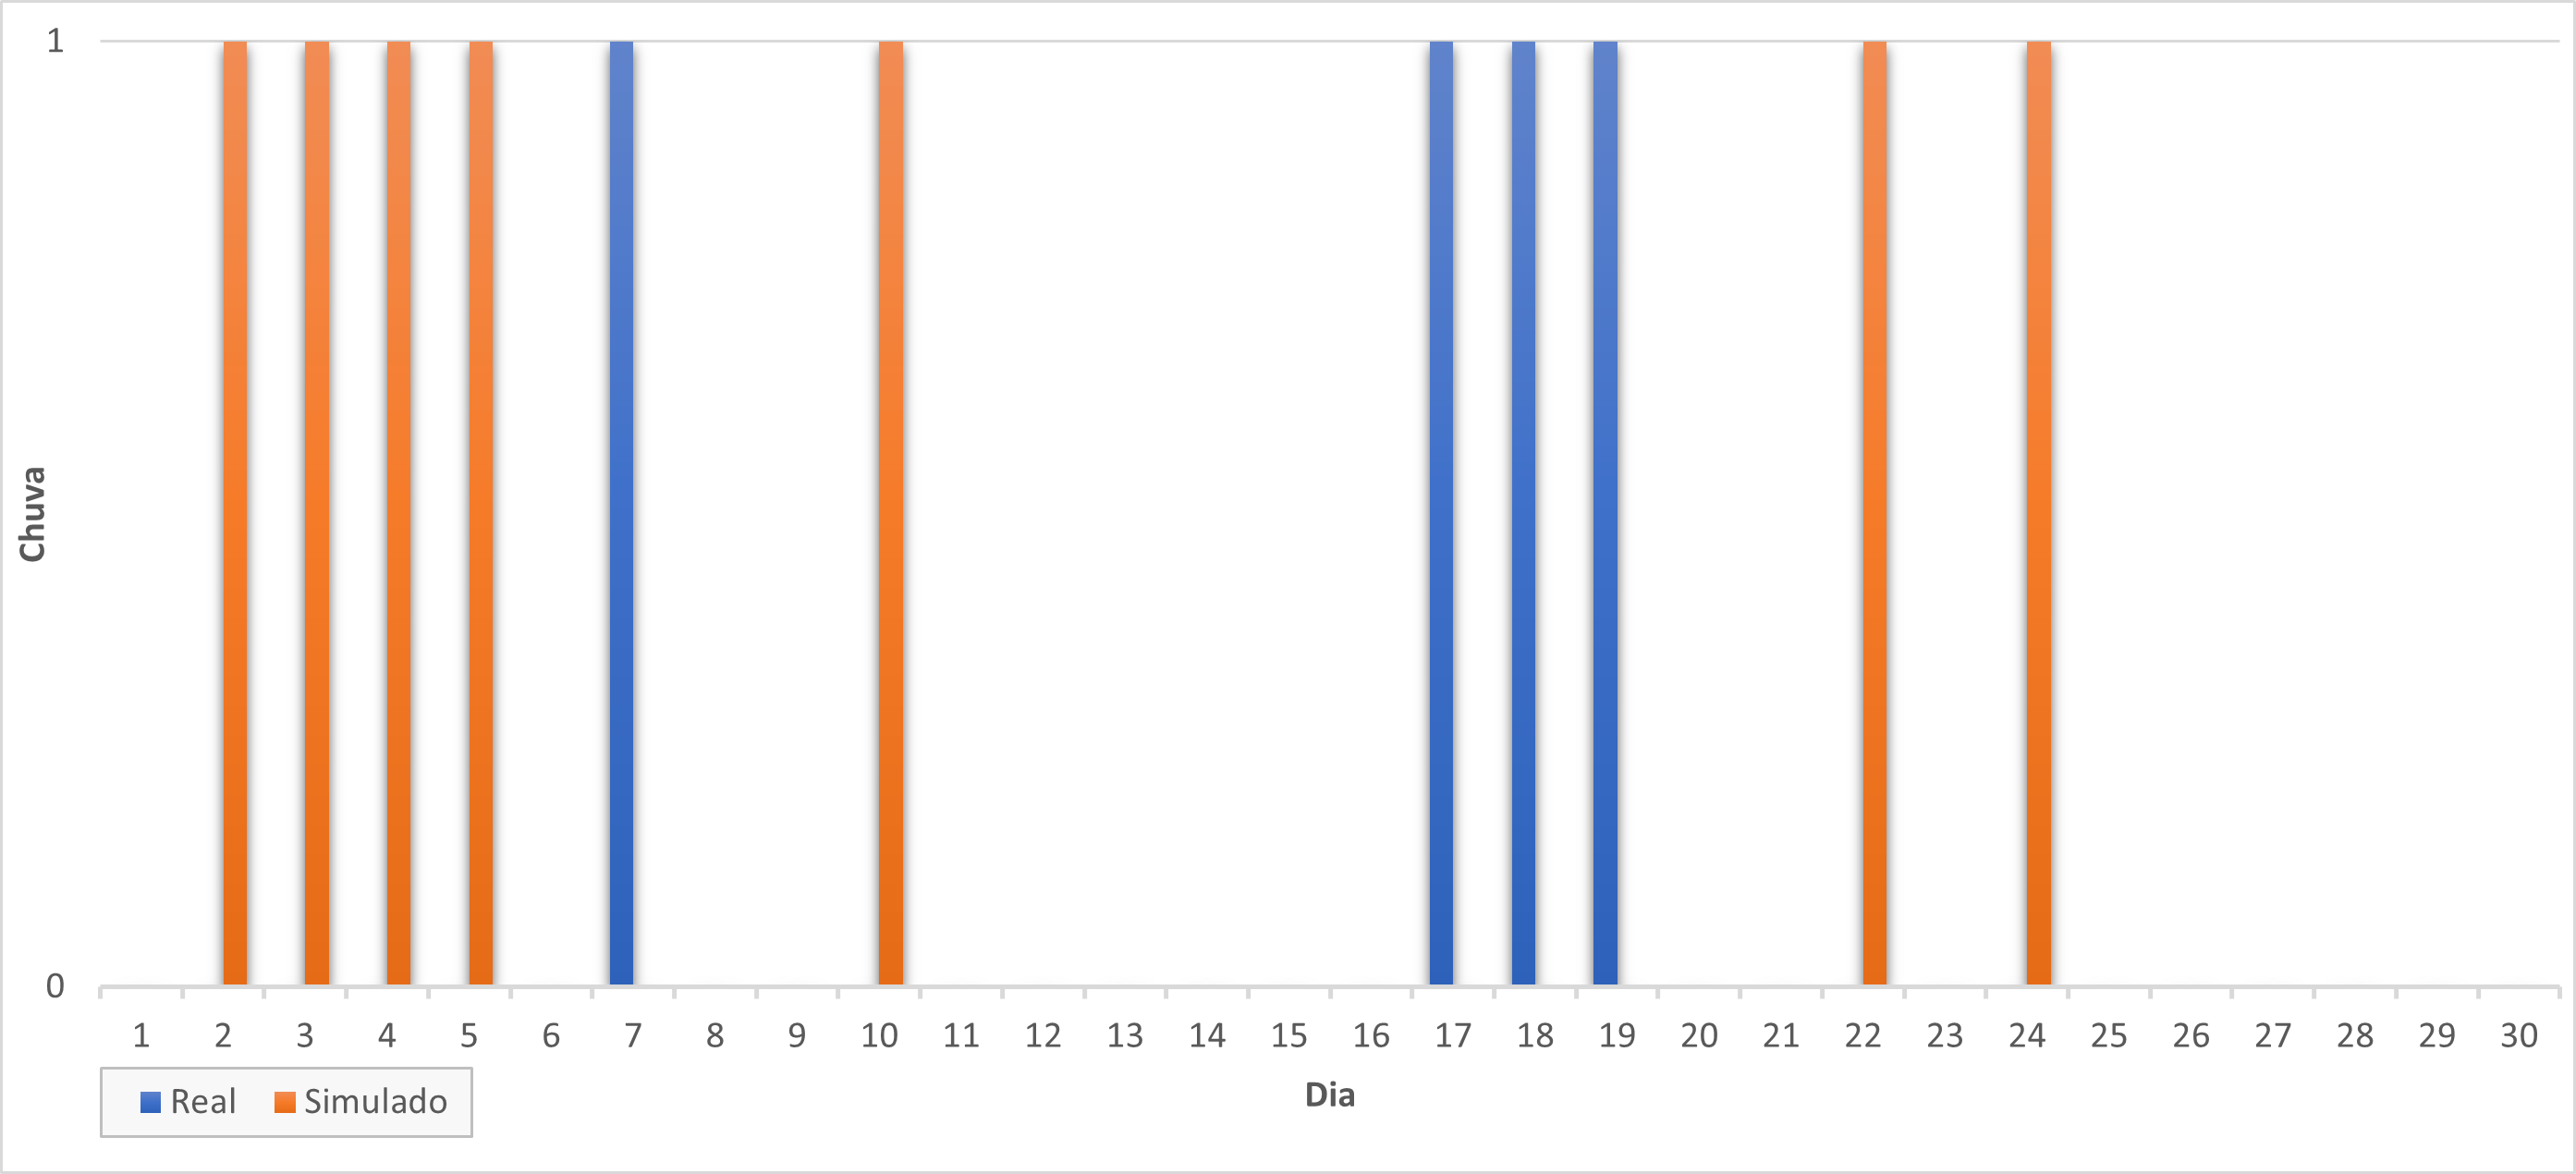
\includegraphics[width=\textwidth]{figs/abr.png}
	\label{f.rabr}
	\legend{\small Fonte: Elaborado pelo autor.}
\end{figure}

\subsection{Maio}
\begin{figure}[H]
	\caption{\small Chuva x Dia - Maio/2021}
	\centering
	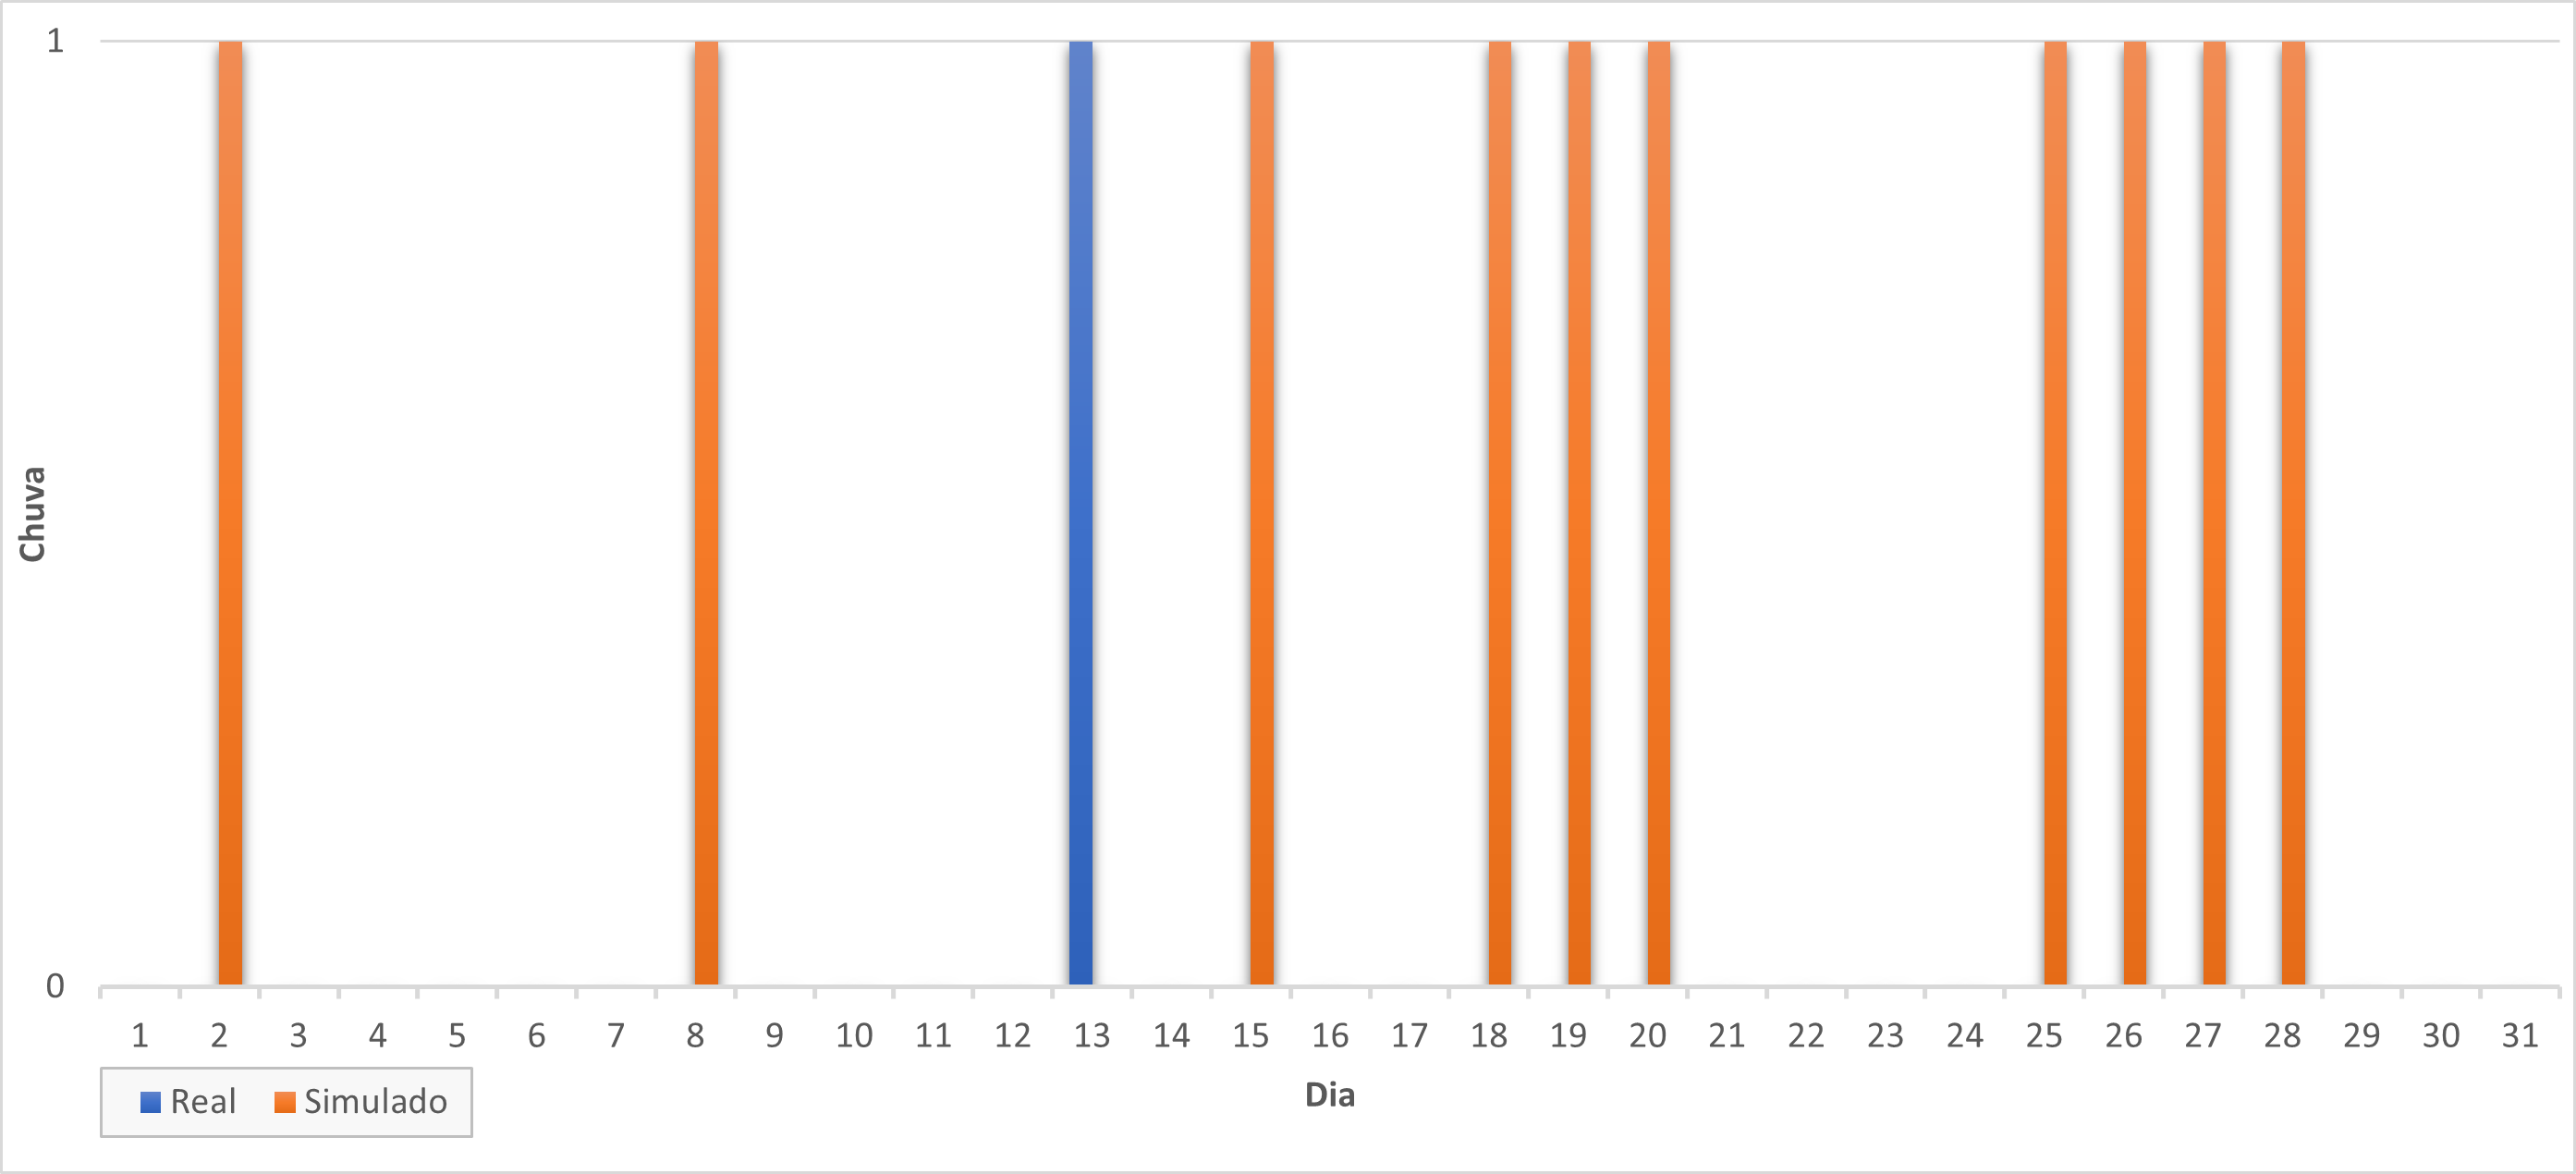
\includegraphics[width=\textwidth]{figs/mai.png}
	\label{f.rmai}
	\legend{\small Fonte: Elaborado pelo autor.}
\end{figure}

\subsection{Junho}
\begin{figure}[H]
	\caption{\small Chuva x Dia - Junho/2021}
	\centering
	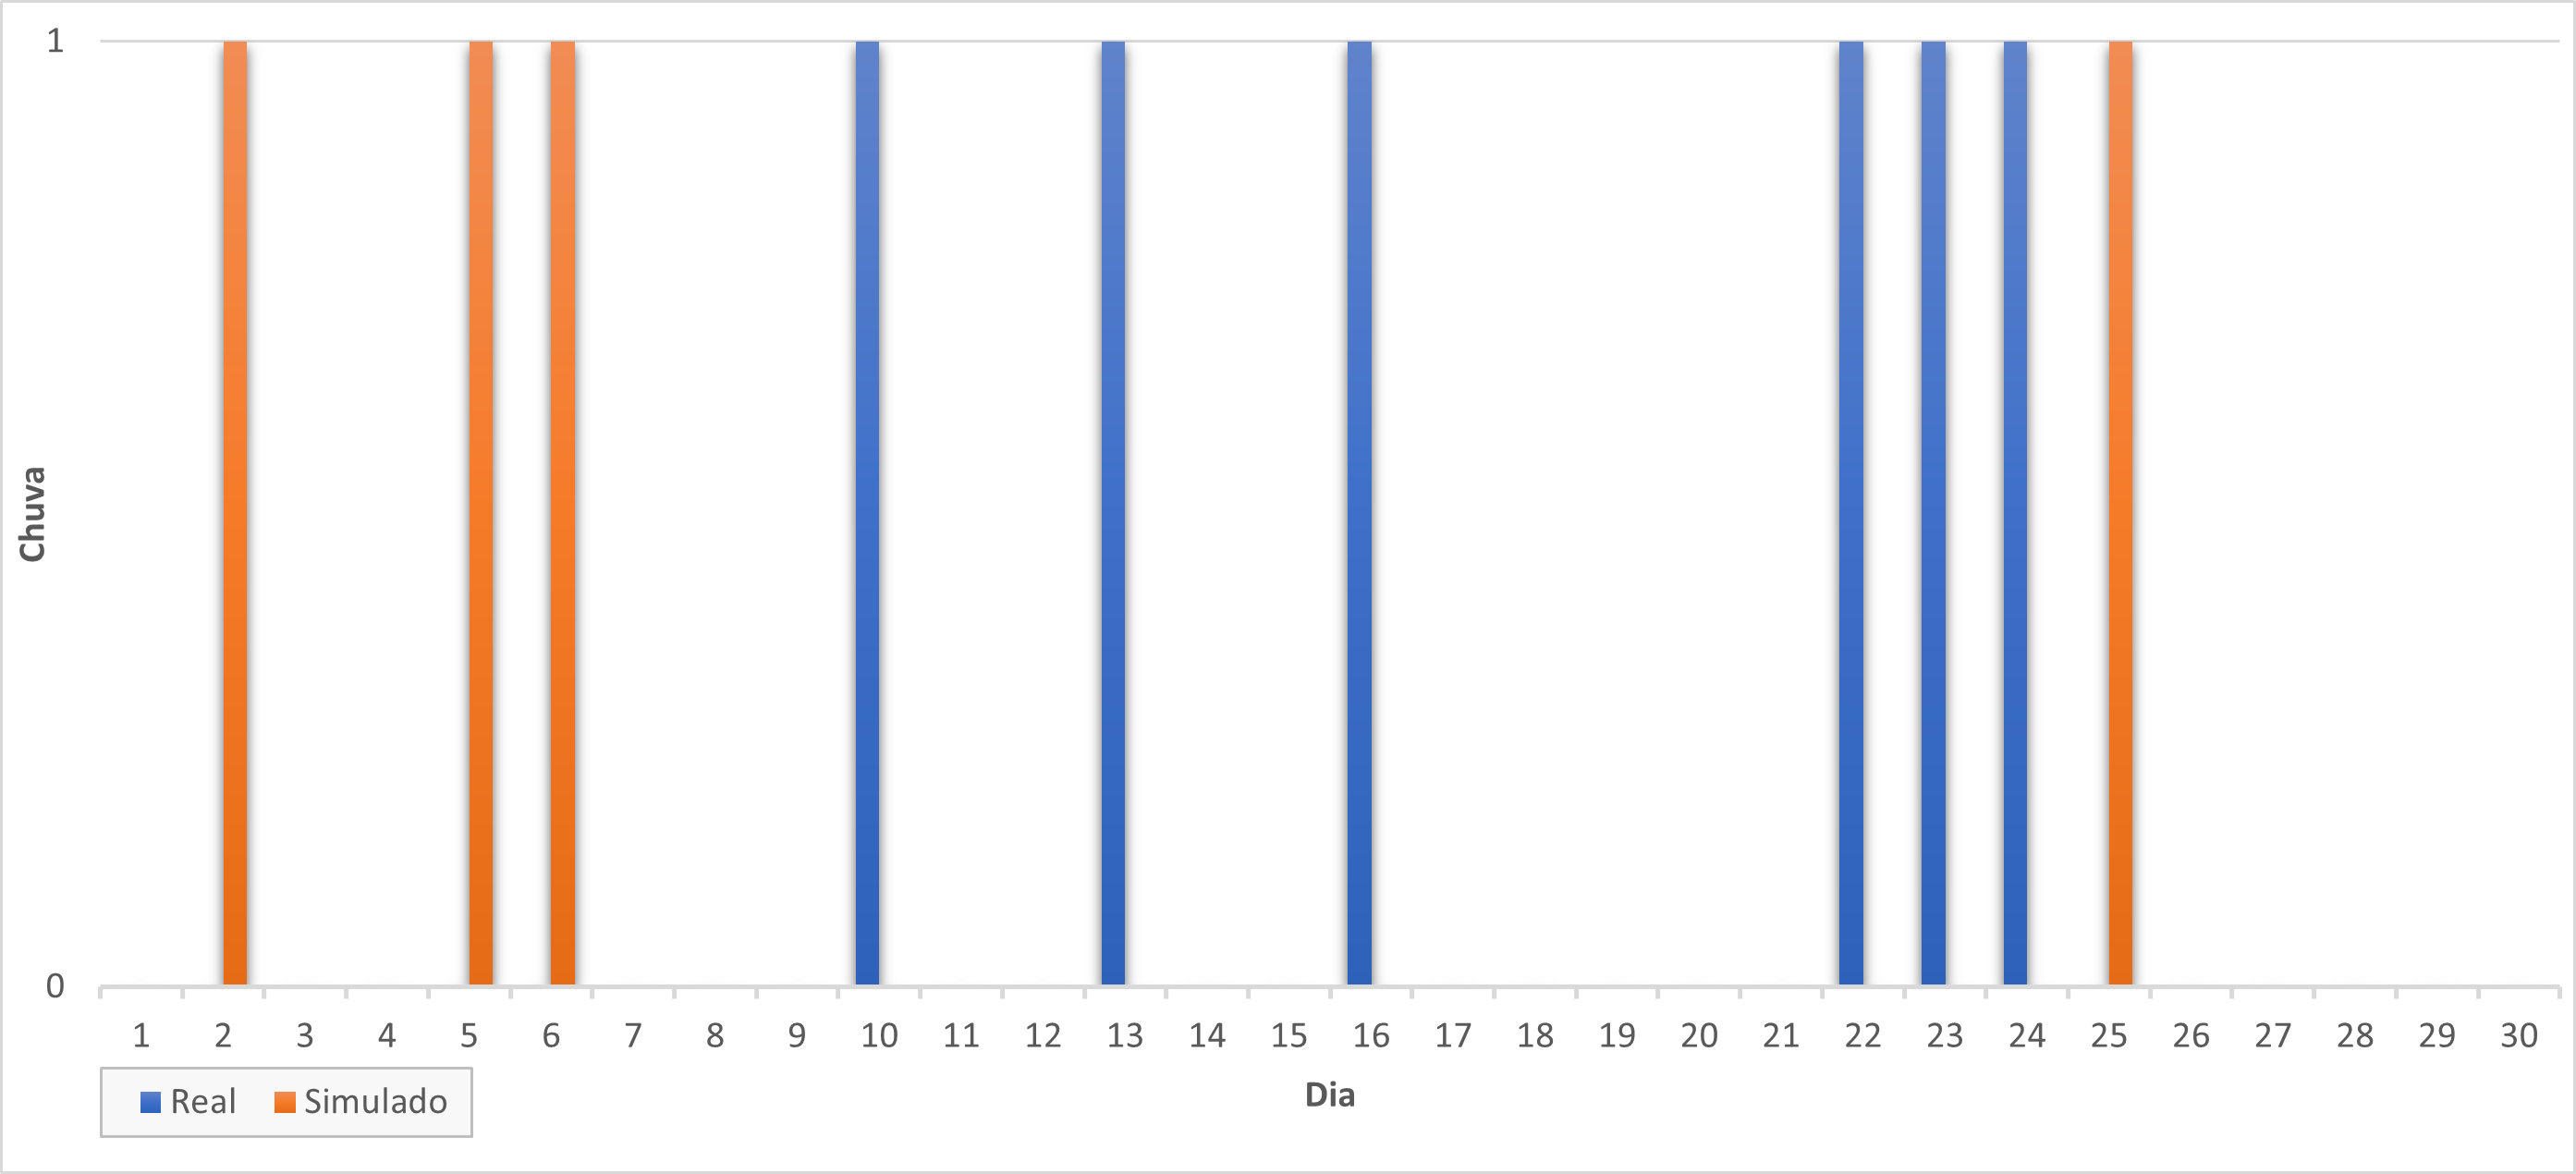
\includegraphics[width=\textwidth]{figs/jun.png}
	\label{f.rjun}
	\legend{\small Fonte: Elaborado pelo autor.}
\end{figure}

\subsection{Julho}
\begin{figure}[H]
	\caption{\small Chuva x Dia - Julho/2021}
	\centering
	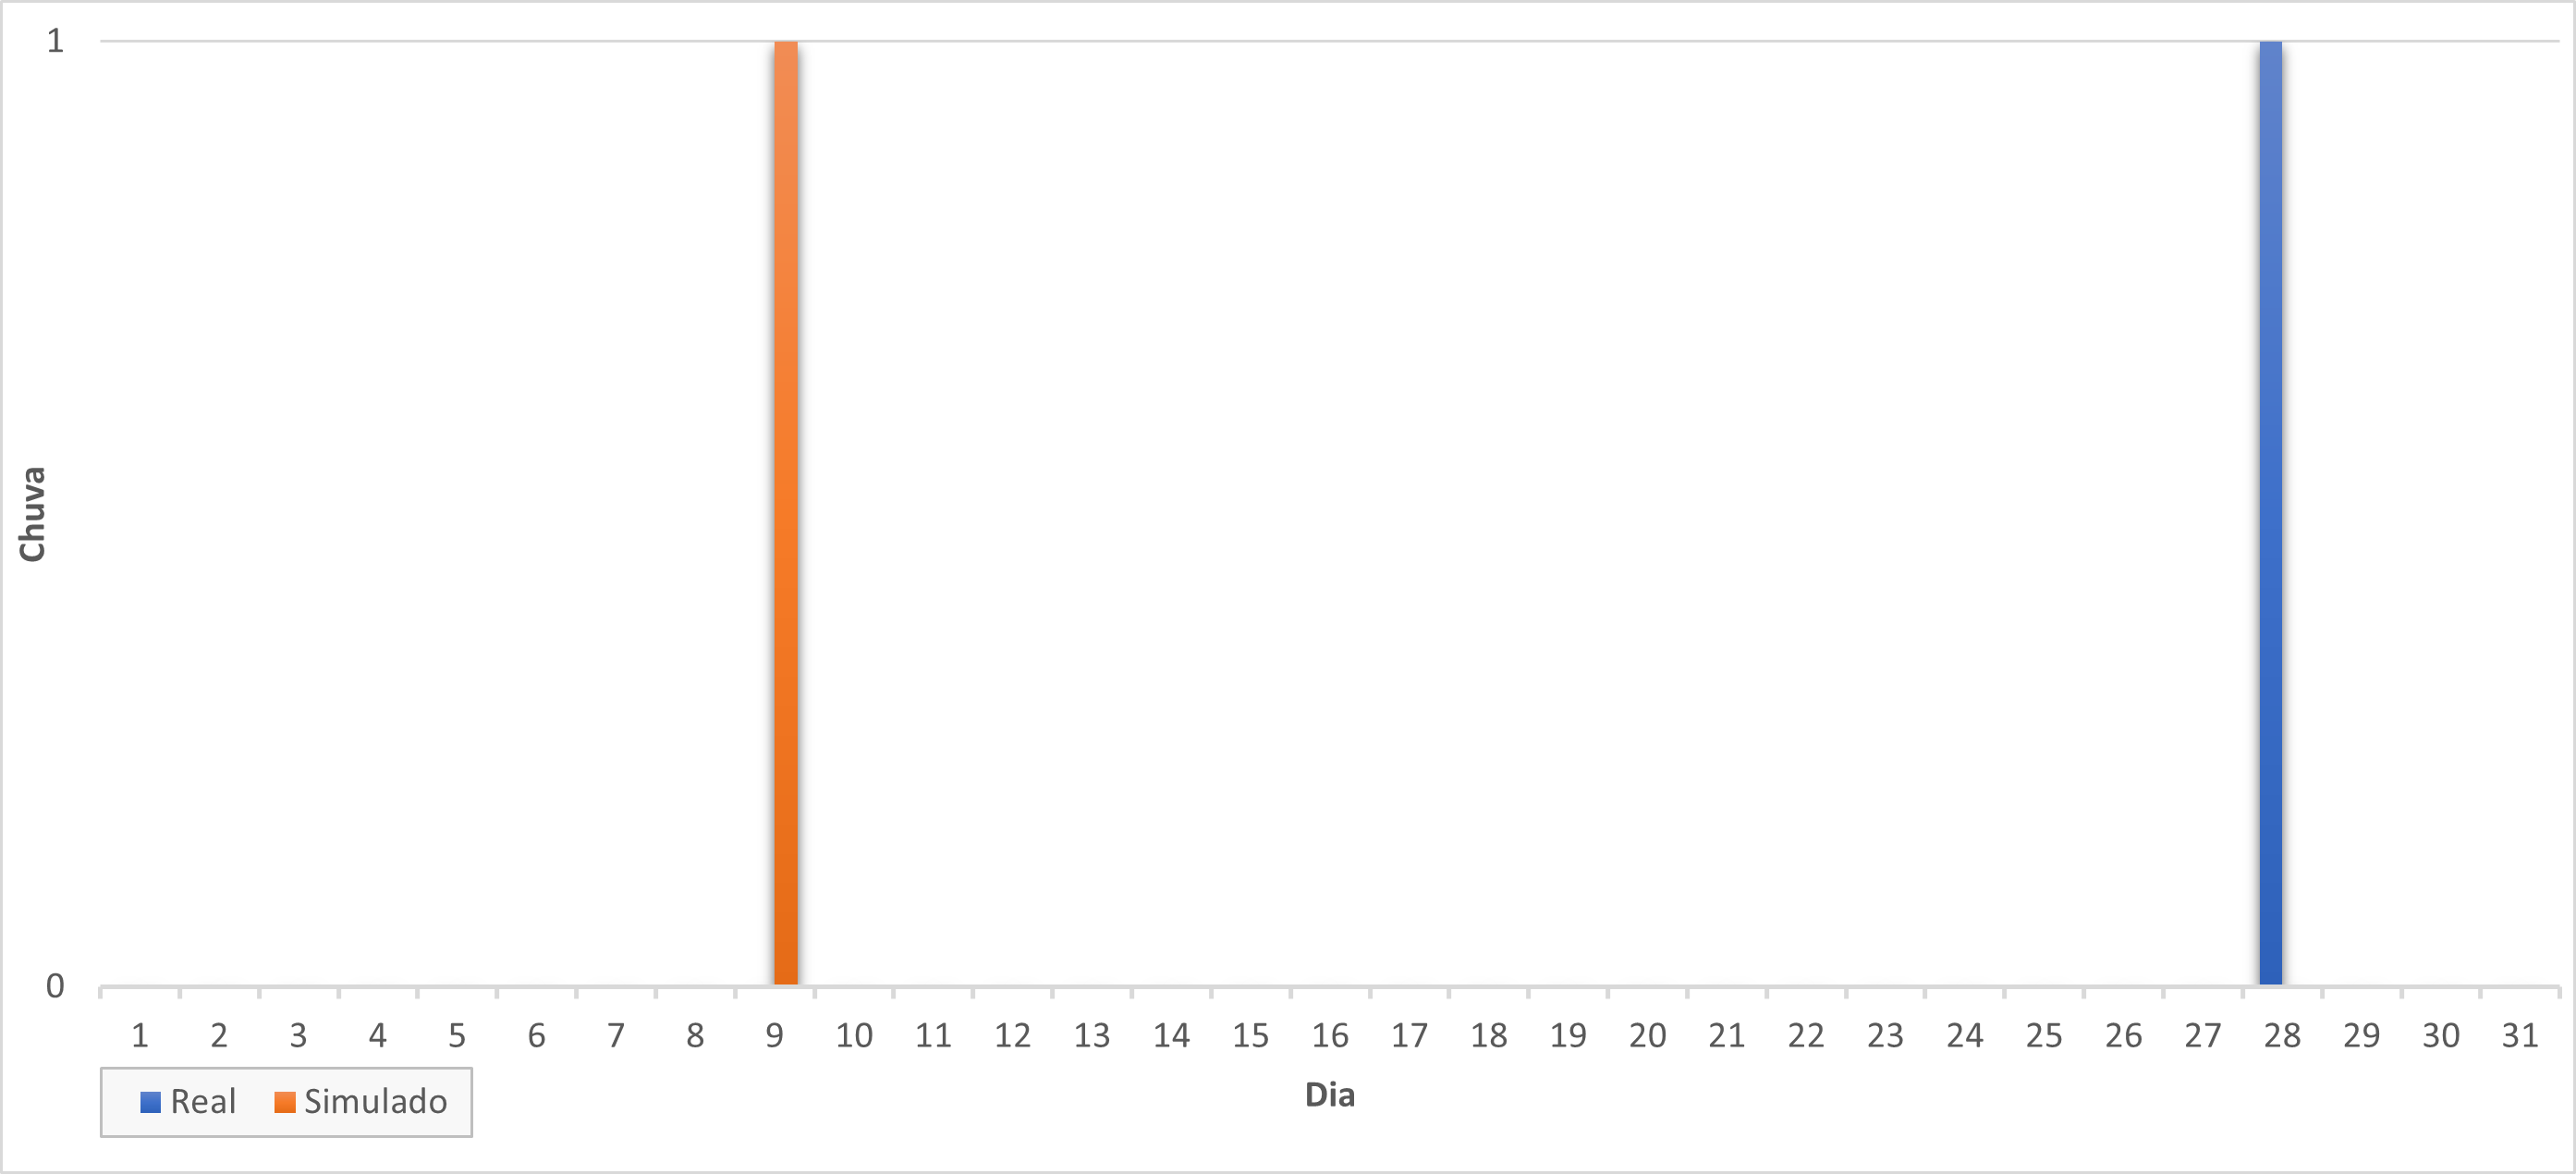
\includegraphics[width=\textwidth]{figs/jul.png}
	\label{f.rjul}
	\legend{\small Fonte: Elaborado pelo autor.}
\end{figure}

\subsection{Agosto}
\begin{figure}[H]
	\caption{\small Chuva x Dia - Agosto/2021}
	\centering
	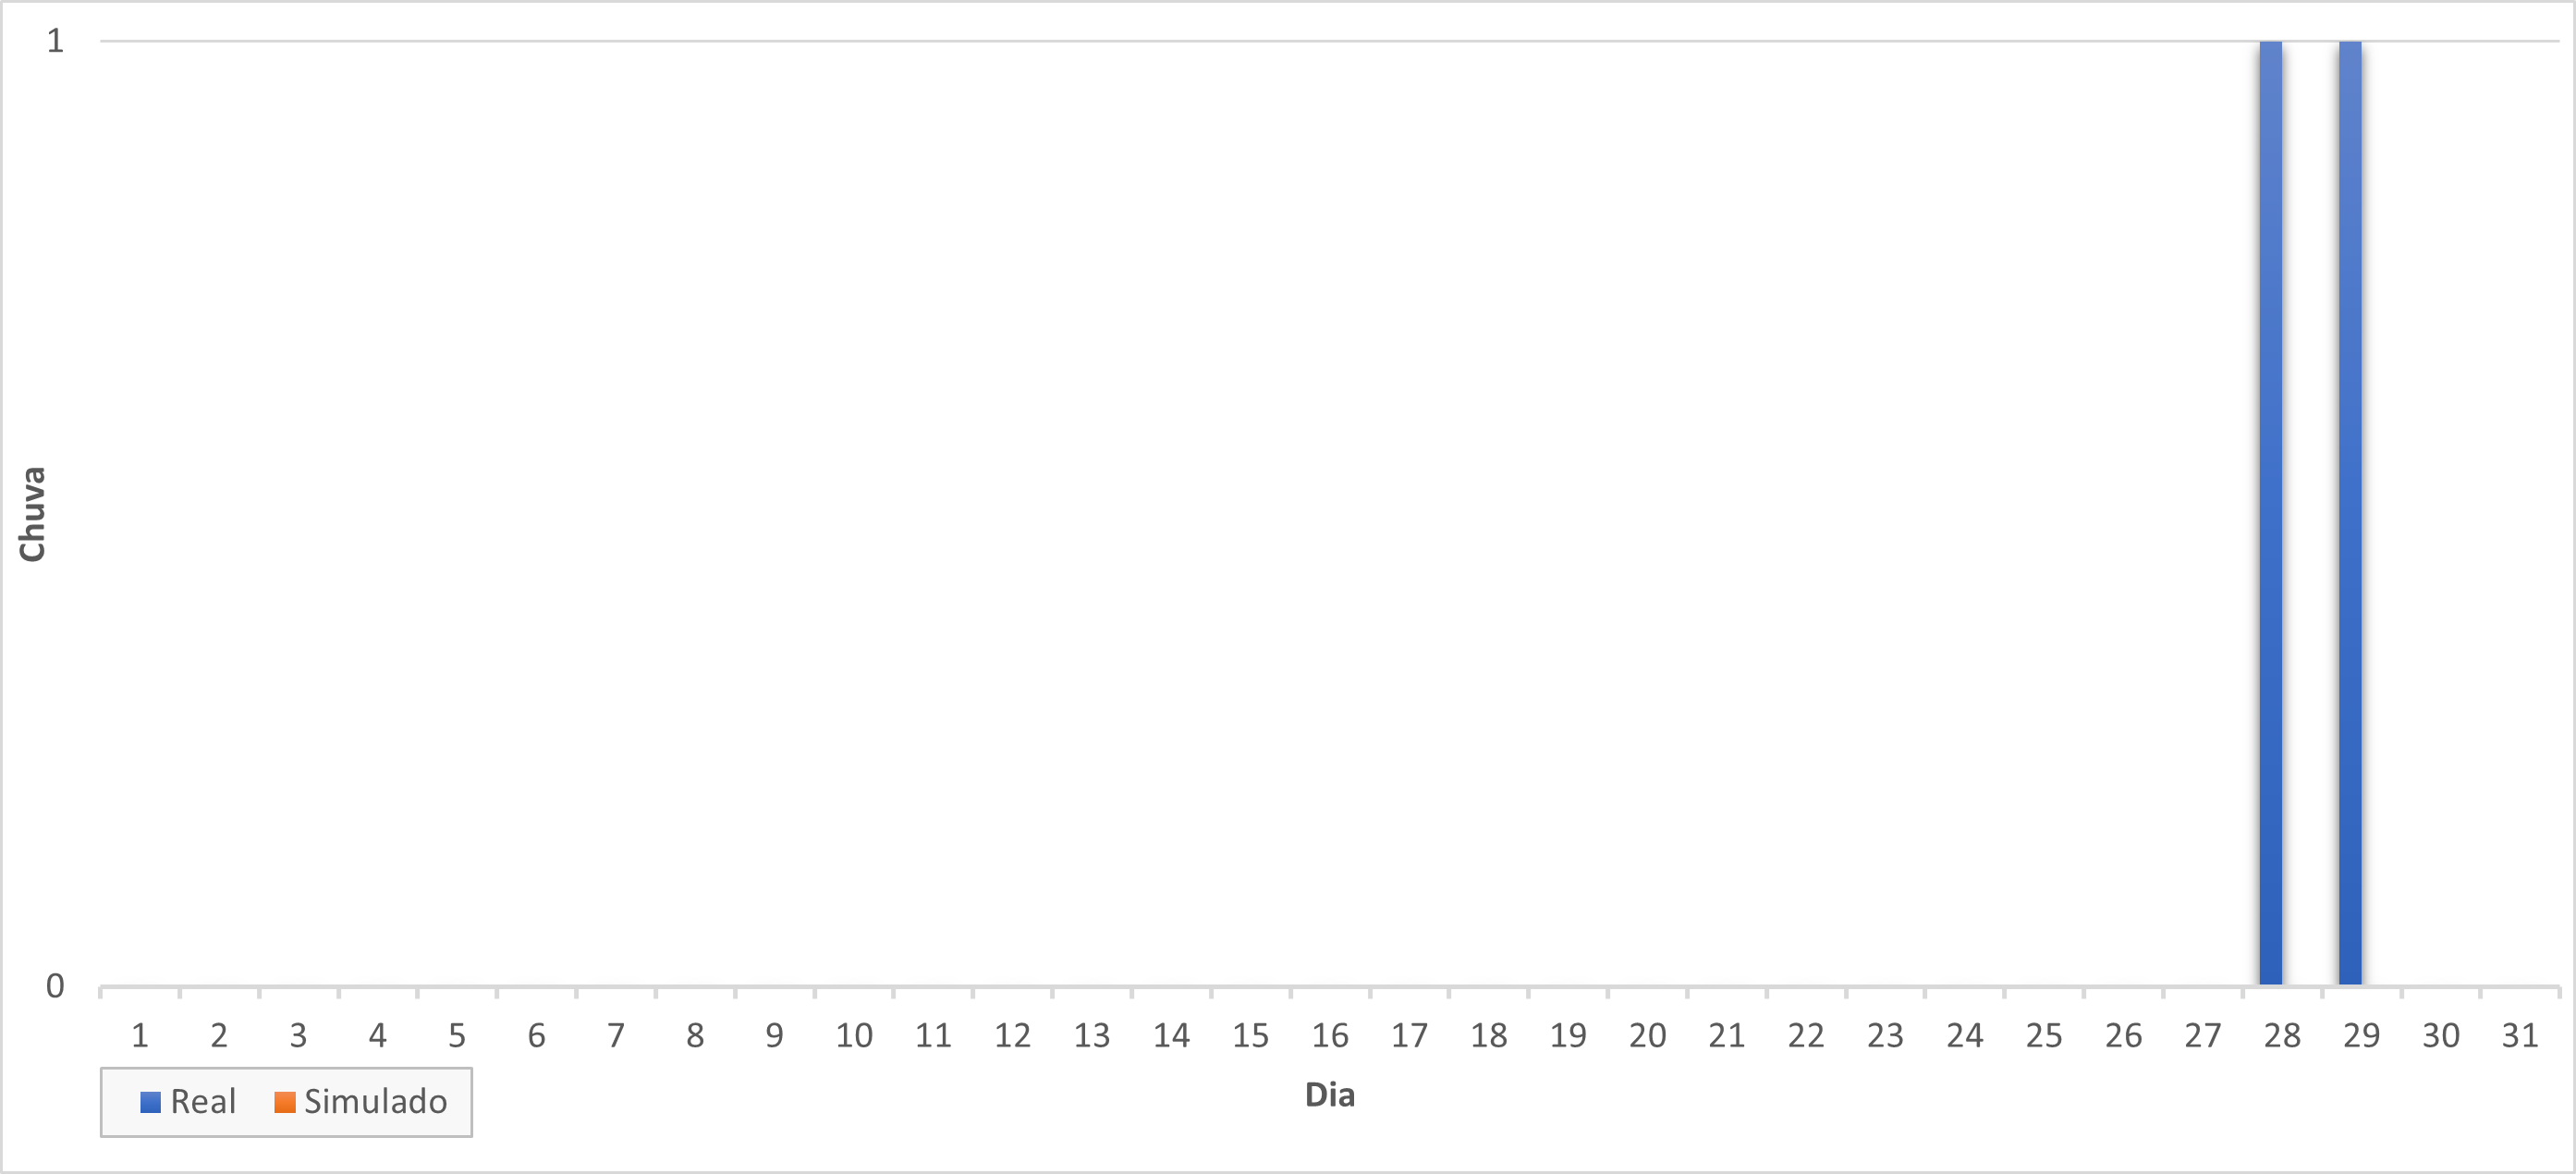
\includegraphics[width=\textwidth]{figs/ago.png}
	\label{f.rago}
	\legend{\small Fonte: Elaborado pelo autor.}
\end{figure}

\subsection{Setembro}
\begin{figure}[H]
	\caption{\small Chuva x Dia - Setembro/2021}
	\centering
	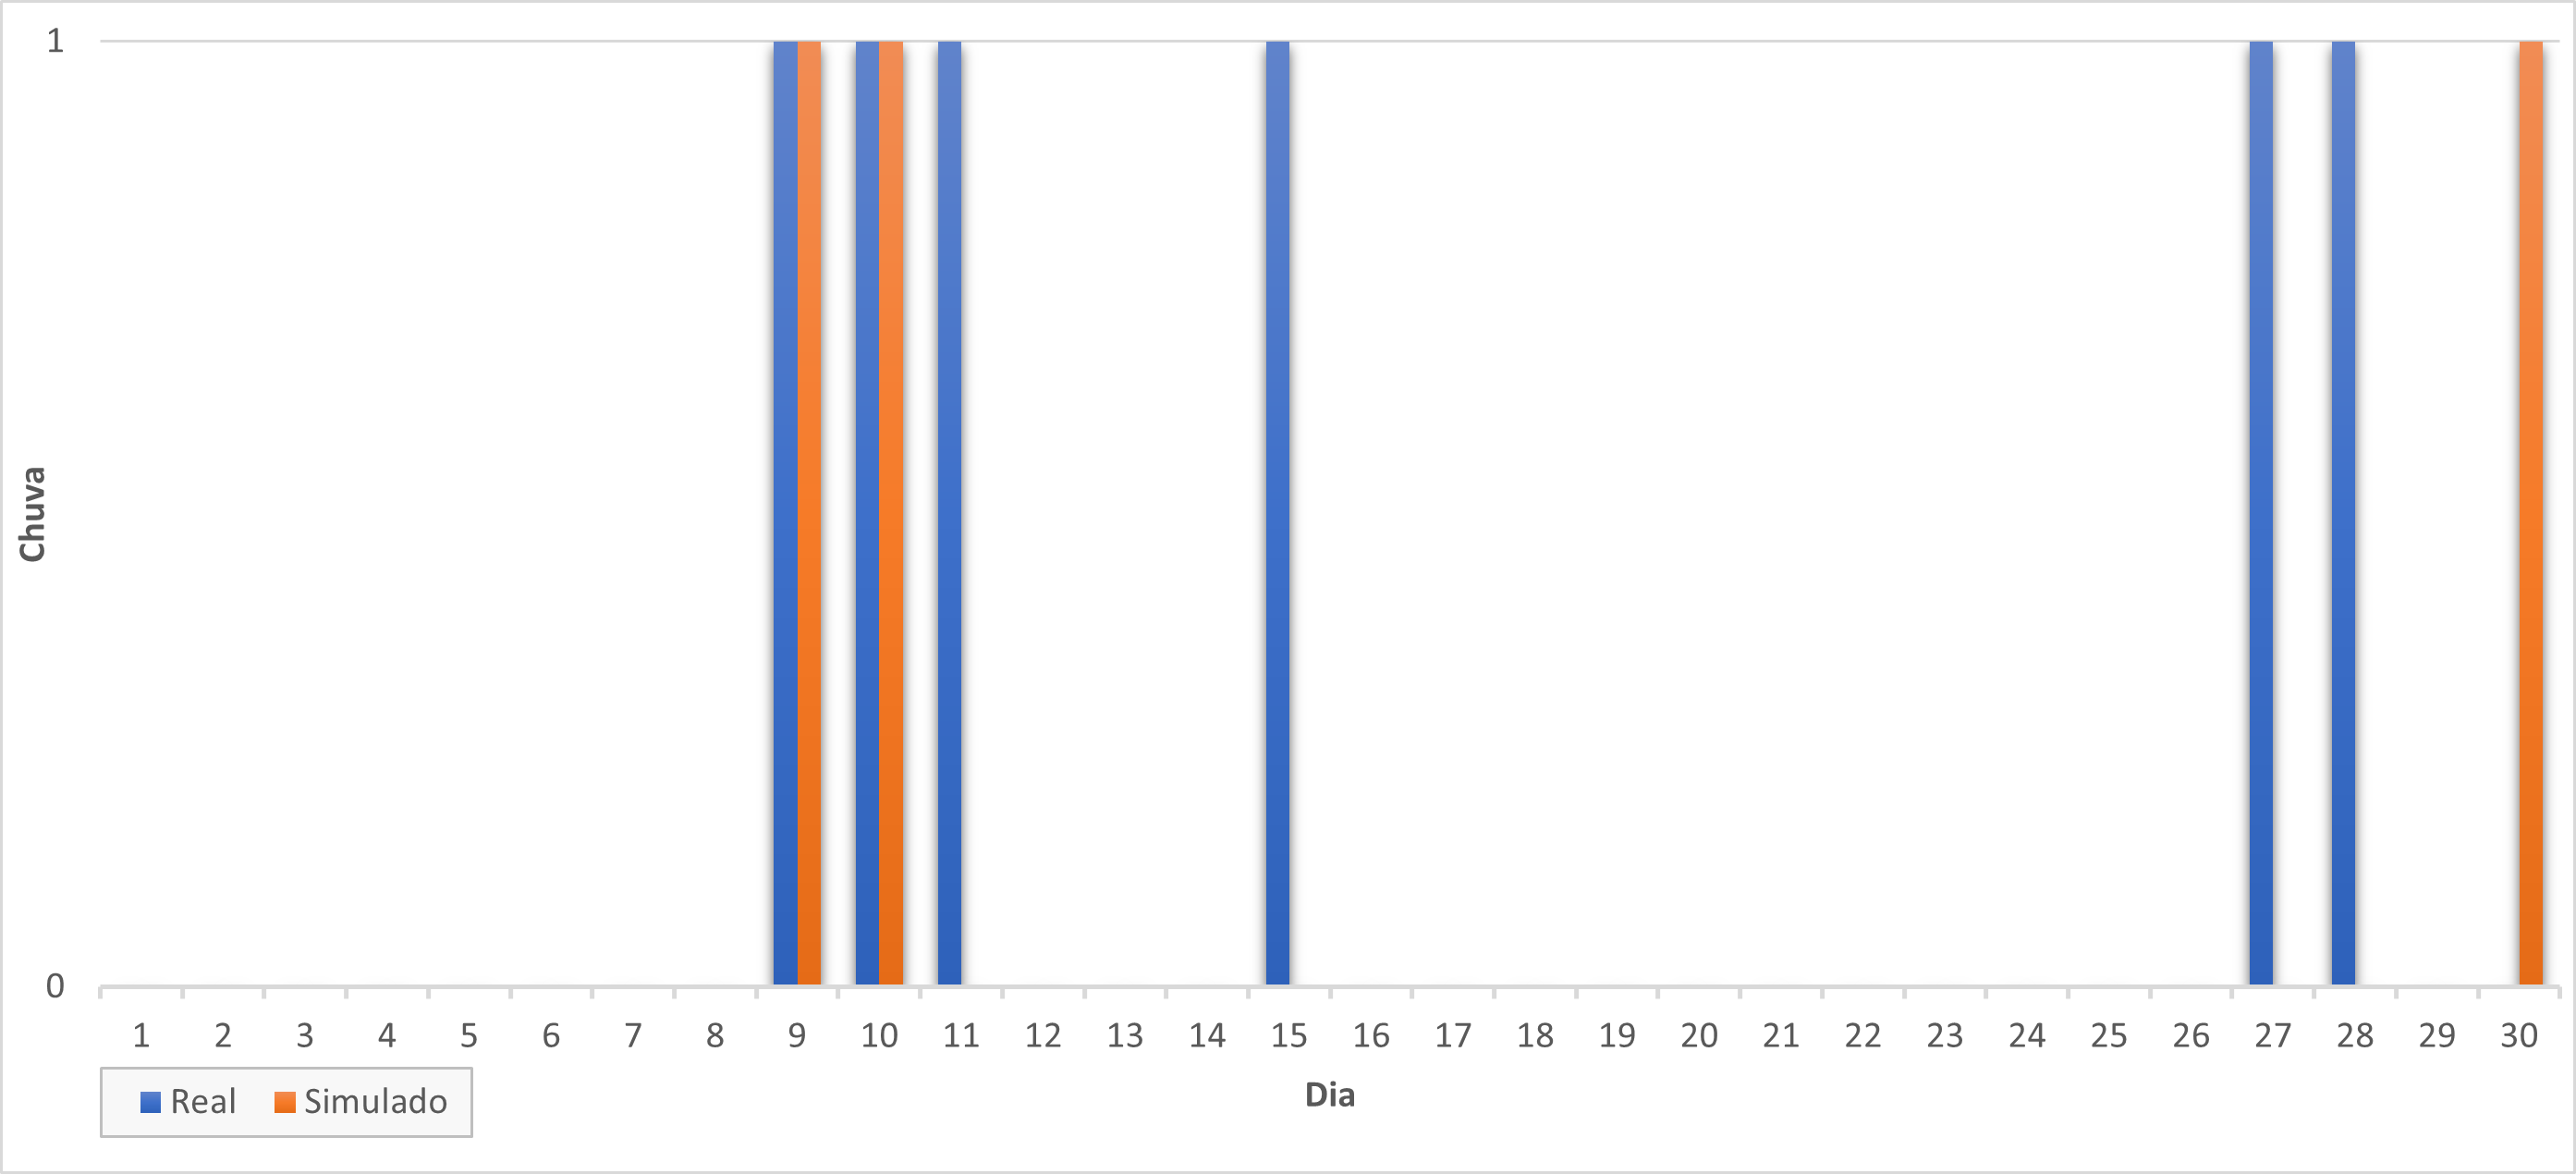
\includegraphics[width=\textwidth]{figs/set.png}
	\label{f.rset}
	\legend{\small Fonte: Elaborado pelo autor.}
\end{figure}

\subsection{Outubro}
\begin{figure}[H]
	\caption{\small Chuva x Dia - Outubro/2021}
	\centering
	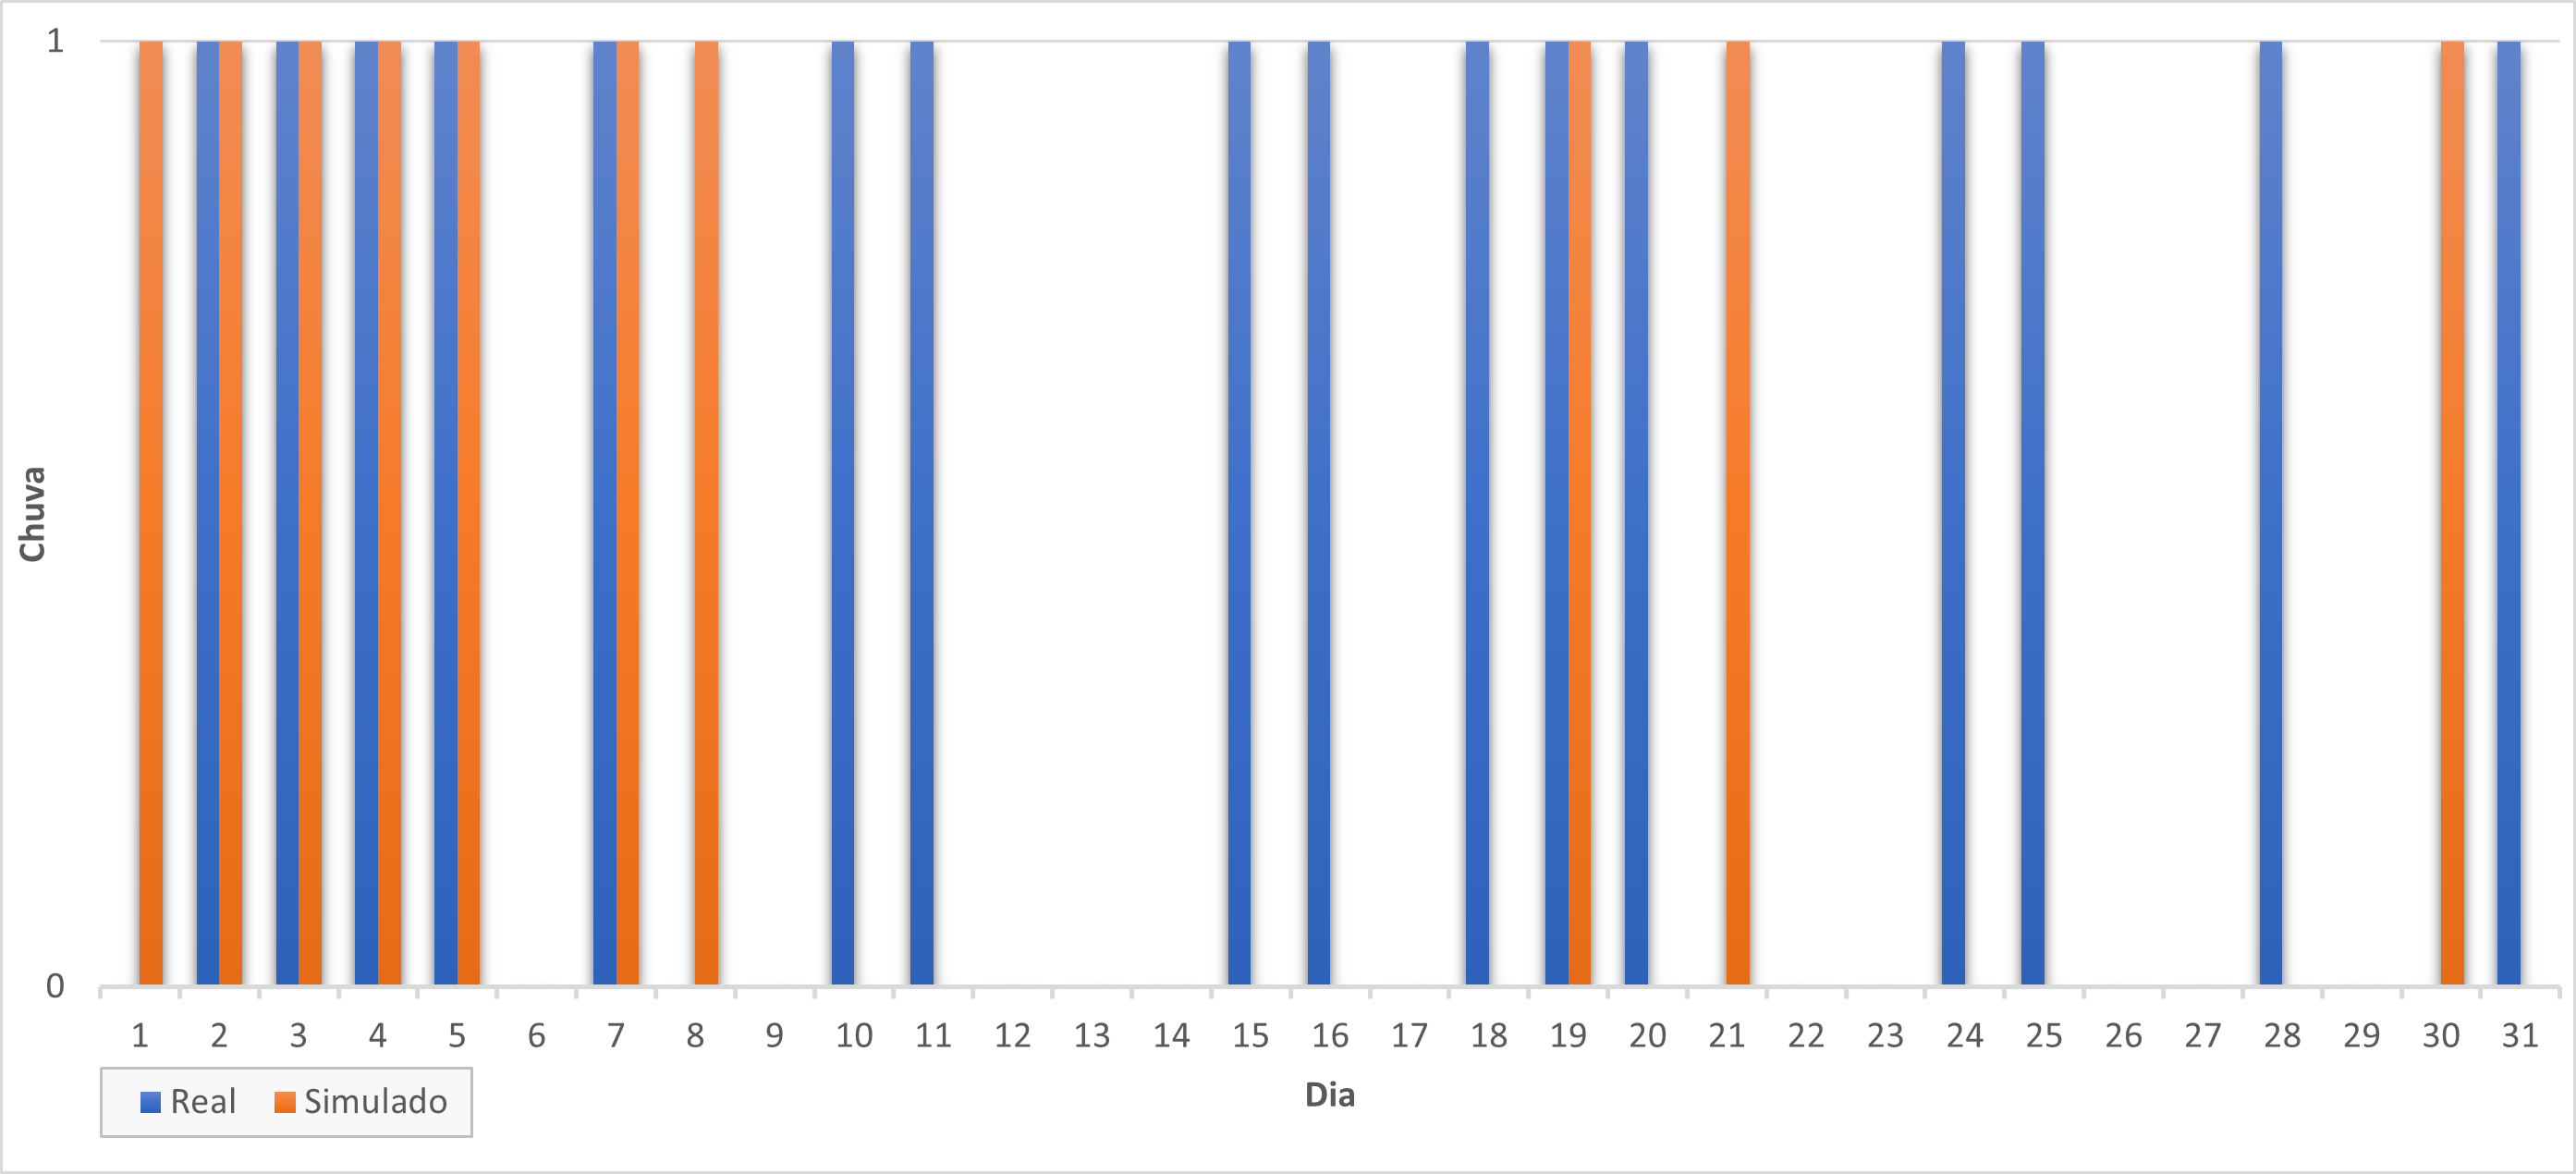
\includegraphics[width=\textwidth]{figs/out.png}
	\label{f.rout}
	\legend{\small Fonte: Elaborado pelo autor.}
\end{figure}

\subsection{Novembro}
\begin{figure}[H]
	\caption{\small Chuva x Dia - Novembro/2021}
	\centering
	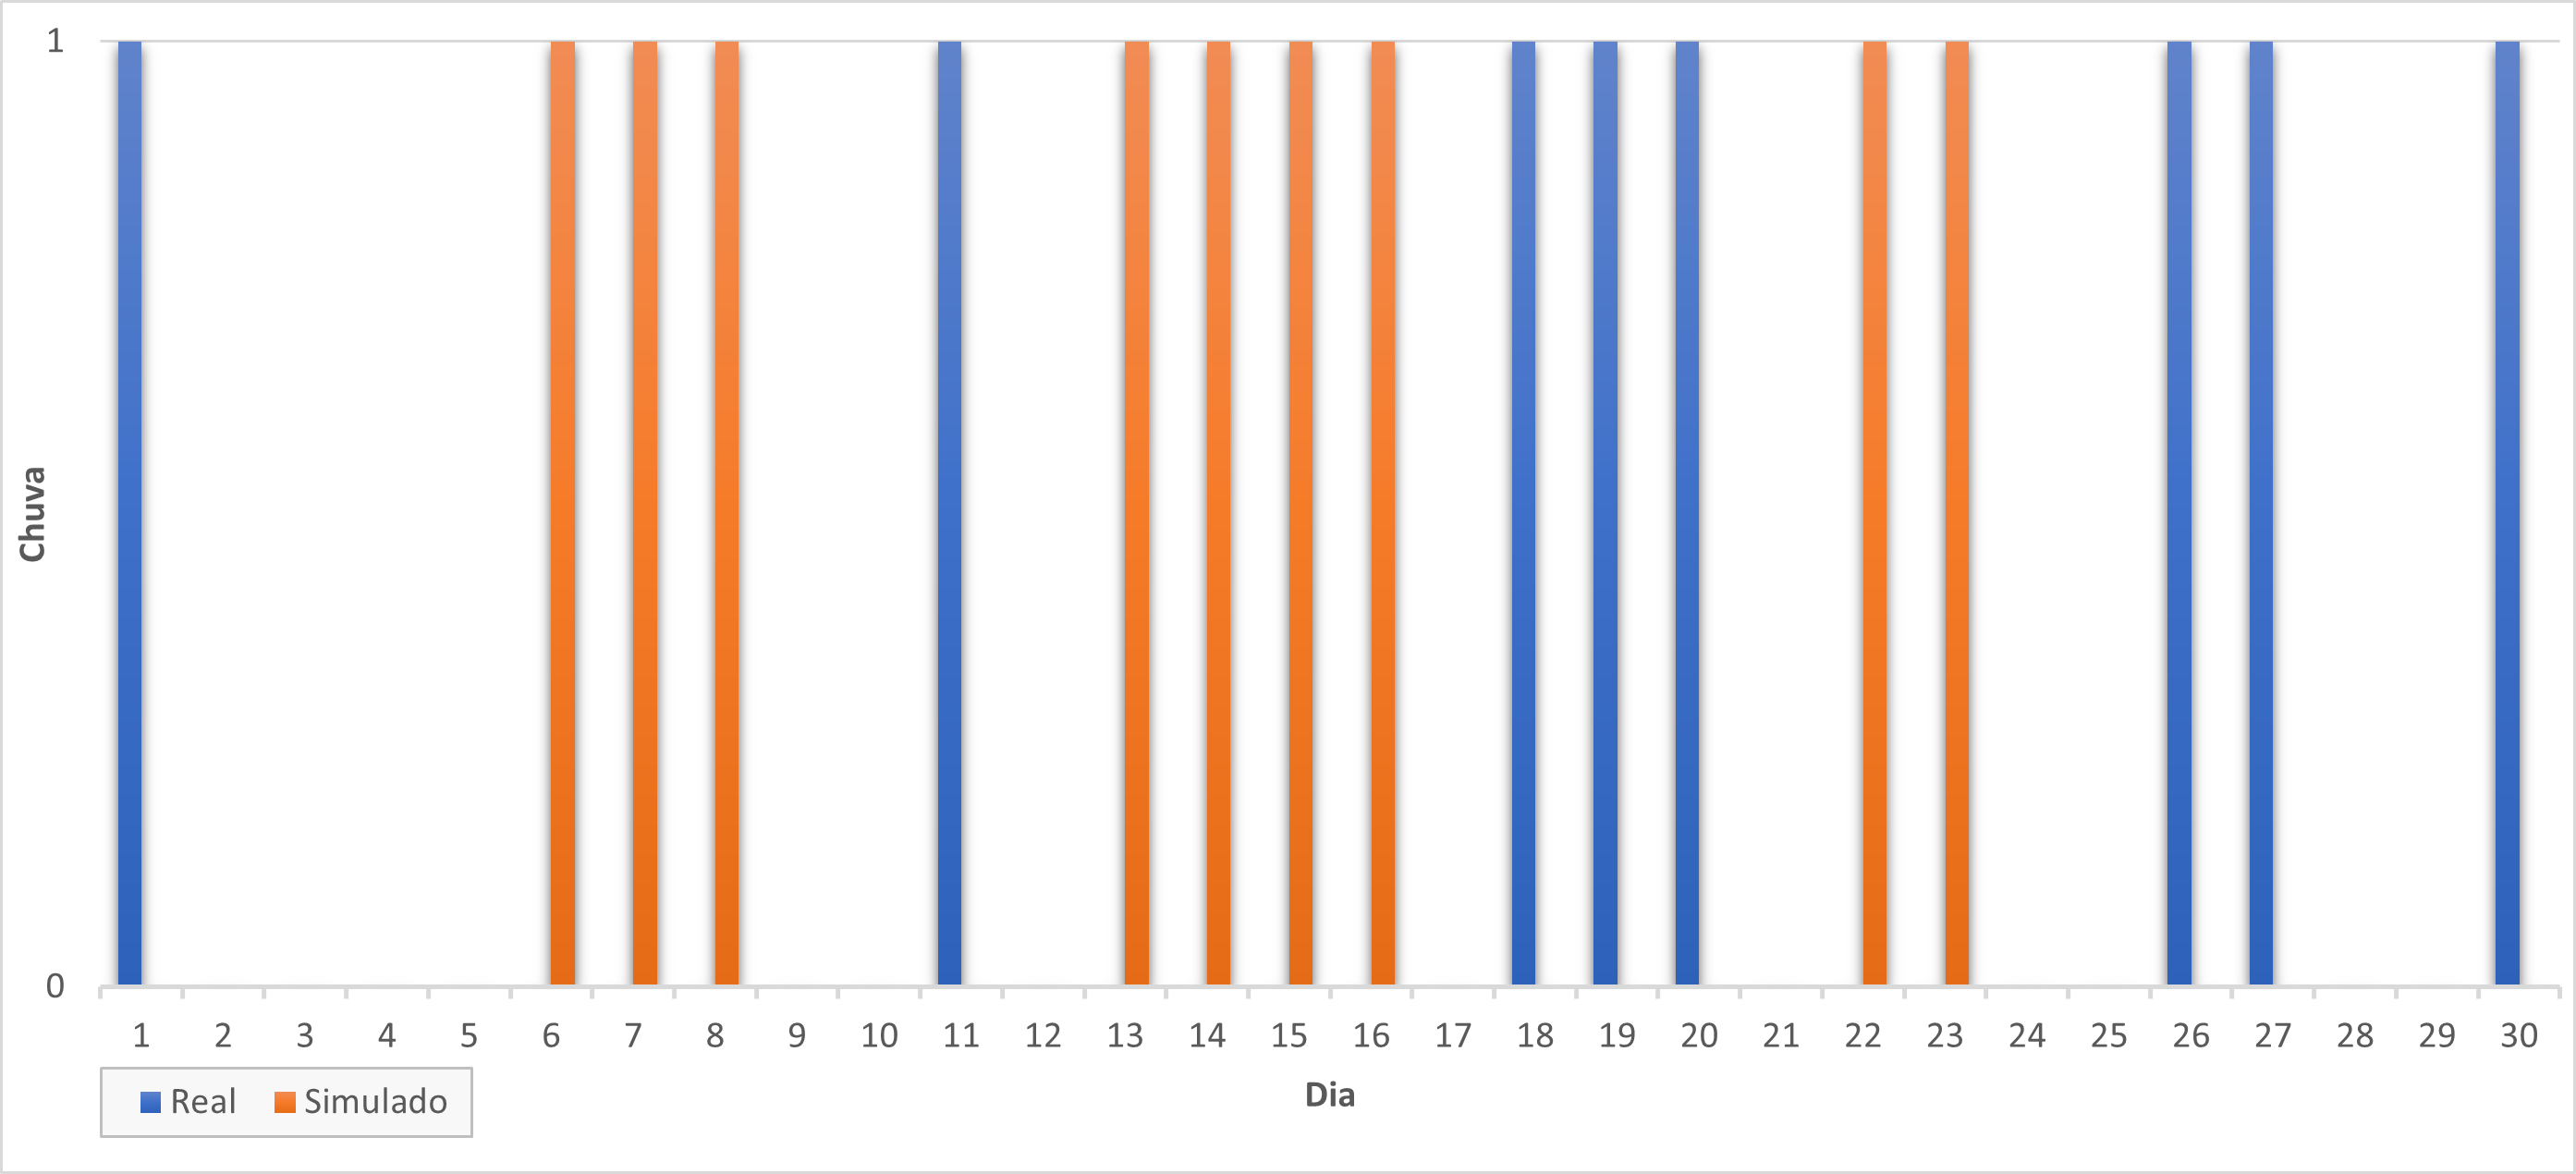
\includegraphics[width=\textwidth]{figs/nov.png}
	\label{f.rnov}
	\legend{\small Fonte: Elaborado pelo autor.}
\end{figure}

\subsection{Dezembro}
\begin{figure}[H]
	\caption{\small Chuva x Dia - Dezembro/2021}
	\centering
	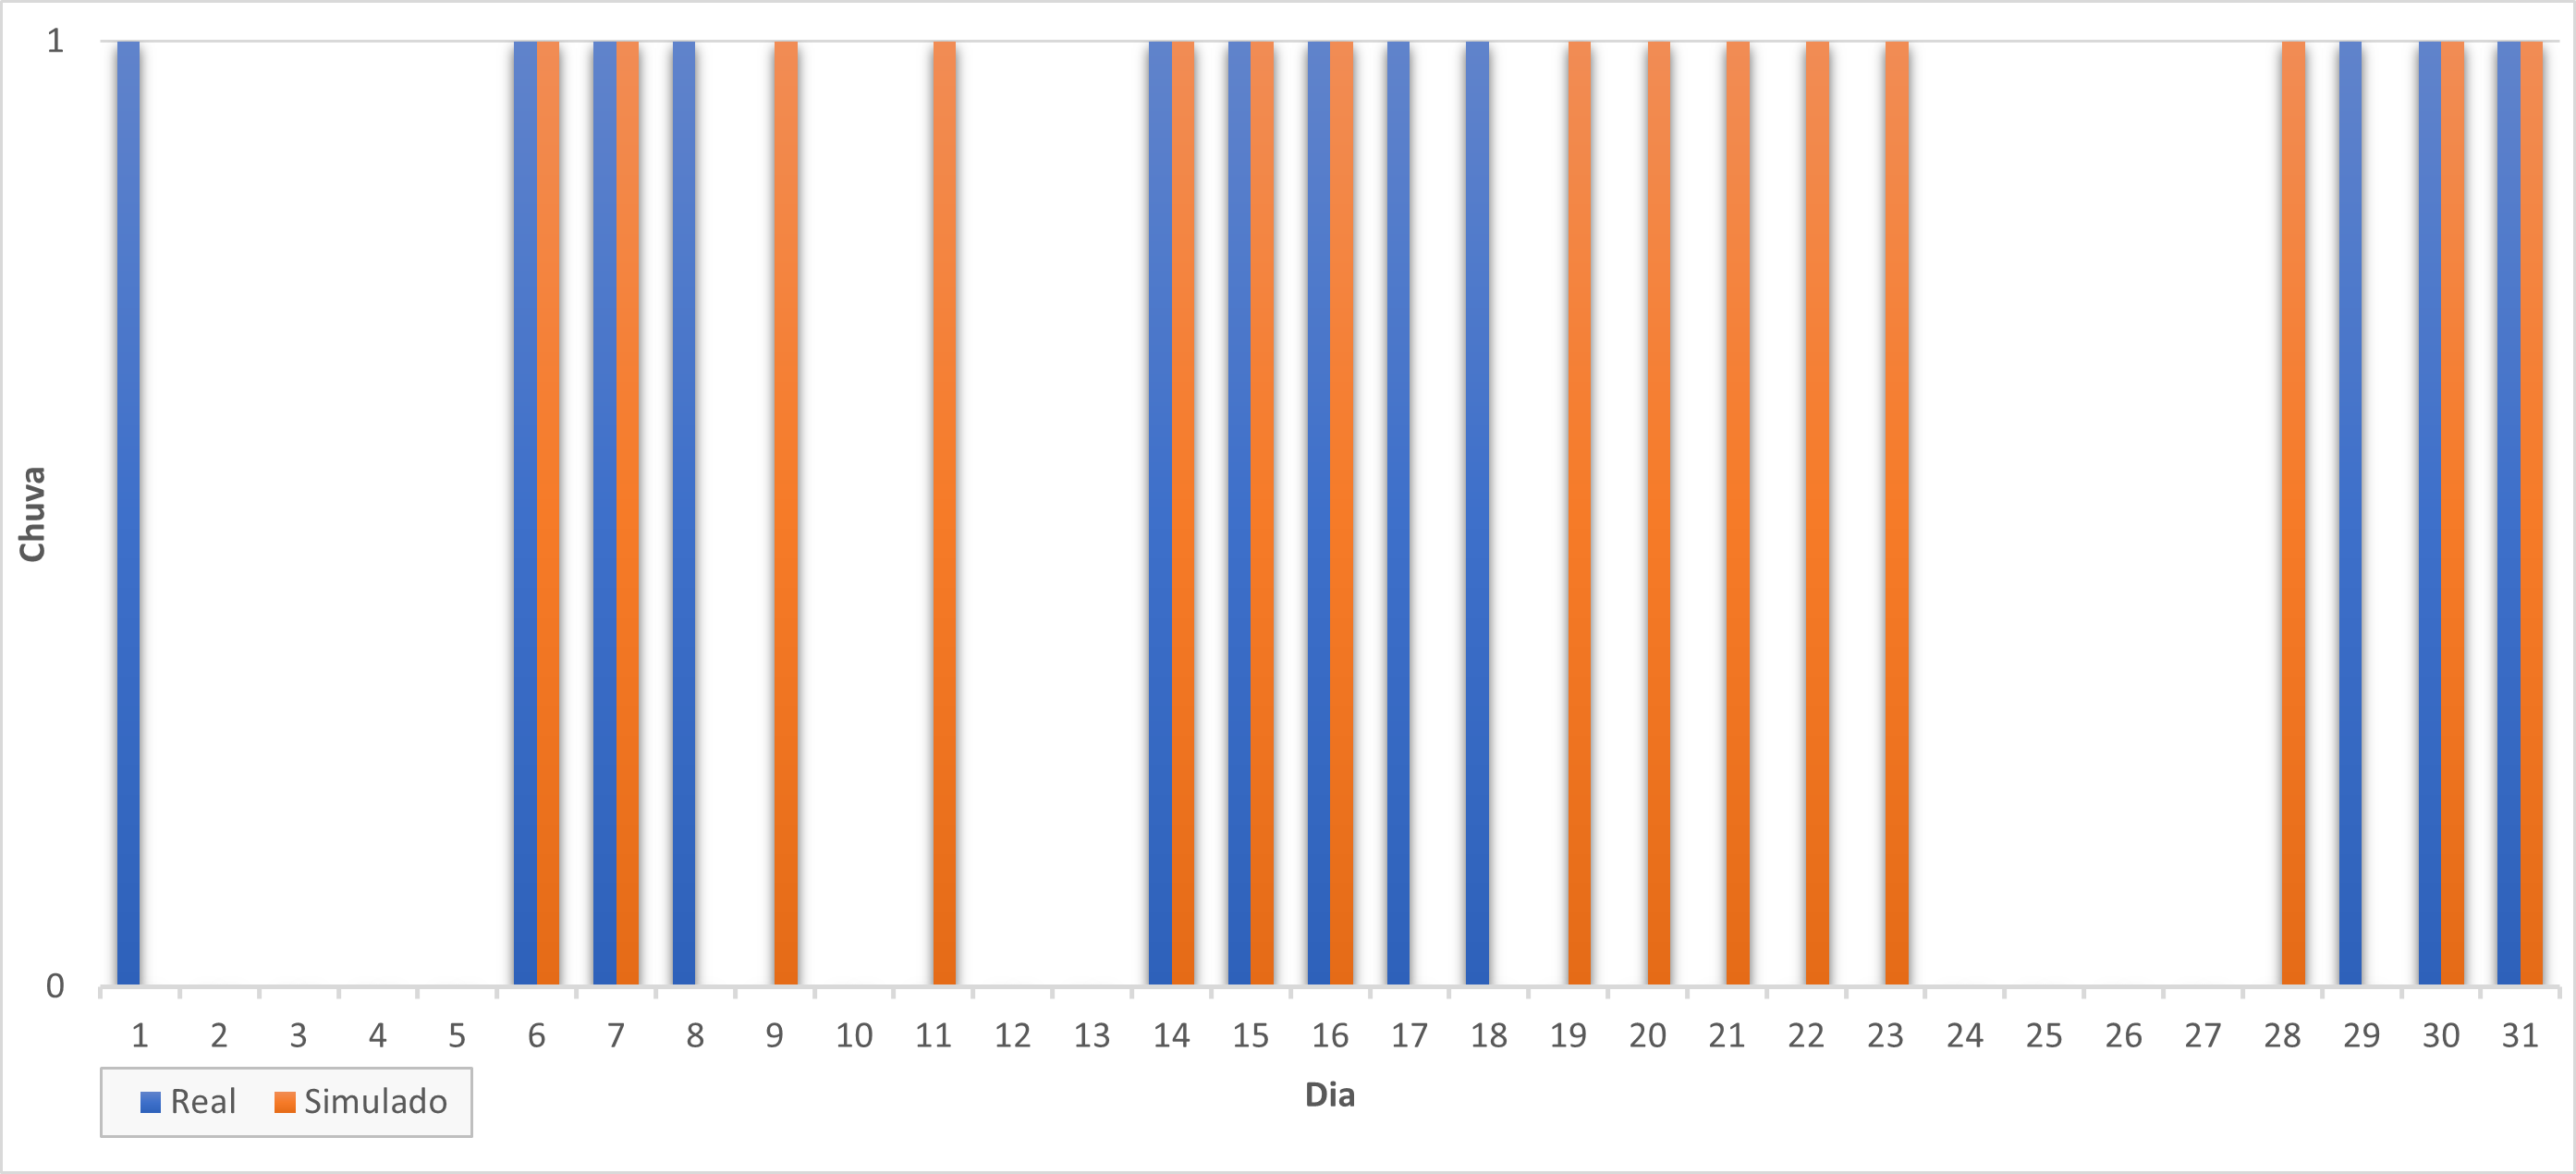
\includegraphics[width=\textwidth]{figs/dez.png}
	\label{f.rdez}
	\legend{\small Fonte: Elaborado pelo autor.}
\end{figure}


\section{Análise do ano inteiro}